\documentclass[UTF8,a4paper]{ctexart}
%###############################################################################
%
%  以下是论文全局环境设置
%
%###############################################################################
%---------------------------------------------------------------------------
% 调整页面
\usepackage{geometry} % 设置页边距,页面大小
\geometry{left=2.5cm,right=2.0cm,top=2.50cm,bottom=2.0cm}
%调整行间距 20 磅
\setlength{\baselineskip}{20pt}
%\linespread{1.3}%调整行间距
\usepackage{setspace} %行间距
\usepackage{array} %
\usepackage{booktabs} %调整表格线与上下内容的间隔
\usepackage{multirow}
\usepackage{hyperref} %加入书签跳转
\usepackage{abstract} % 修改摘要

%---------------------------------------------------------------------------
%正文页眉页脚设定
\pagestyle{plain}    % 没有页眉,页脚是居中的页码;
\usepackage{fancyhdr}
\pagestyle{fancy}
\fancyhf{}
\lhead{} \chead{华北电力大学本科毕业设计(论文)} \rhead{}
\lfoot{} \cfoot{~\thepage~} \rfoot{}

%---------------------------------------------------------------------------
% 设置字体
%\usepackage[fontset=windows]{ctex}
\usepackage{fontspec} %引入字体Times New Roman字体
\setmainfont{Nimbus Roman}
%\setmainfont{Times New Roman}             %设置正文字体为Times New Roman
\usepackage{xeCJK} %调用系统中已安装的字体
\setCJKmainfont{SimSun}
%% 支持汉字加粗
\let\heiti\relax % 黑体
\newCJKfontfamily\heiti{SimHei}[AutoFakeBold]
\setCJKsansfont{SimHei}[AutoFakeBold]

\let\songti\relax % 宋体
\newCJKfontfamily\songti{SimSun}[AutoFakeBold]
\setCJKmainfont{SimSun}[AutoFakeBold]  

%% 设置字体大小


%---------------------------------------------------------------------------
%% 目录格式设置
\usepackage{tocloft}      %必须这么写,否则会报错
\renewcommand{\contentsname}{\centerline{\Large{\heiti{目\quad\quad 录}}}}
%\renewcommand{\cftchapleader}{\cftdotfill{0.6}} %设置chapter条目的引导点间距
\renewcommand{\cftsecleader}{\cftdotfill{0.6}}
\renewcommand{\cftsubsecleader}{\cftdotfill{0.6}}
\renewcommand{\cftsubsubsecleader}{\cftdotfill{0.6}}
%\renewcommand{\cftchapfont}{\hts}    %设置chapter条目的字体
\renewcommand{\cftsecfont}{\heiti\large}    %设置section条目的字体
\renewcommand{\cftsubsecfont}{\songti\large} %设置subsection条目的字体
\renewcommand{\cftsubsubsecfont}{\songti\large} %设置subsection条目的字体

%---------------------------------------------------------------------------
% 数学公式
\usepackage{amsmath}
\usepackage{mathtools}
\numberwithin{equation}{section}
\renewcommand\theequation{%
    \thesection - \arabic{equation}}

%---------------------------------------------------------------------------
% 插入代码块
\usepackage{listings}
\usepackage{xcolor}
\lstset{
 %language=bash,                % the language of the code
 columns=fixed,       
% numbers=left,                                        % 在左侧显示行号
% numberstyle=\tiny\color{gray},                       % 设定行号格式
 frame=none,                                          % 不显示背景边框
 backgroundcolor=\color[RGB]{245,245,244},            % 设定背景颜色
 keywordstyle=\color[RGB]{40,40,255},                 % 设定关键字颜色
 numberstyle=\footnotesize\color{darkgray},           
 commentstyle=\it\color[RGB]{0,96,96},                % 设置代码注释的格式
% stringstyle=\rmfamily\slshape\color[RGB]{128,0,0},   % 设置字符串格式
}

%---------------------------------------------------------------------------
% 图表操作
\usepackage{graphicx} % 引入图片
%\usepackage[justification=centering]{caption} % 图片的caption居中
\usepackage[indent]{caption} % 设置图片的 caption 换行缩进
%% Inkscape矢量图
\usepackage{import}
\usepackage{xifthen}
\usepackage{pdfpages}
\usepackage{transparent}
\usepackage{calc} %调整大小
%% 修改图表
\usepackage{float} %修改表格的位置
\usepackage{makecell} %表格类换行
\usepackage{booktabs} %加粗表格线

%% 表格和图片编号
\makeatletter

\numberwithin{figure}{section}
\renewcommand{\thefigure}{\thesection - \arabic{figure}}

\numberwithin{table}{section}
\renewcommand{\thetable}{\thesection - \arabic{table}}
%\renewcommand{\thetable}{\ifnum \c@section>\z@ \thesection-\fi \@arabic\c@table}
\makeatother

%% 图表去除冒号
\usepackage{caption}
\captionsetup[table]{labelsep=space}
\captionsetup[figure]{labelsep=space}

%% 表格和图片标题字体设置
%\usepackage{etoolbox}
%\AtBeginEnvironment{tabular}{\Huge}
\captionsetup{font={normalsize}}


%% 表格小数点对齐
\usepackage{dcolumn}
\newcolumntype{d}{D{.}{.}{2}}

%---------------------------------------------------------------------------
%插入pdf
\usepackage{pdfpages}

%---------------------------------------------------------------------------
% 参考文献格式设置
\usepackage{cite}
%引用多个参考文献
\usepackage[numbers,sort&compress]{natbib}
\newcommand\citeup[1]{{\setcitestyle{square,super}\cite{#1}}}
%\renewcommand\refname{\centering\heiti\zihao{-2}{参考文献}}

%---------------------------------------------------------------------------
%%%%定制标题样式
%%%%% section
\CTEXsetup[name={第,章 },format={\centering\heiti\zihao{-2}},aftername={\enspace},beforeskip={24bp},afterskip={18bp}]{section} %name选项中不要使用中文逗号 \zihao(-2)字号小二
%%%%% subsection
\CTEXsetup[format={\raggedright\songti\zihao{-3}},aftername={\enspace},beforeskip={24bp},afterskip={6bp}]{subsection}
%%%%% subsubsection
\CTEXsetup[format={\raggedright\songti\zihao{4}},aftername={\enspace},beforeskip={12bp},afterskip={6bp}]{subsubsection}


%###############################################################################
%
%  以下是论文内容结构
%
%###############################################################################
%--------------------------------------------------------------------------------
\begin{document}\zihao{-4}
%% 封面
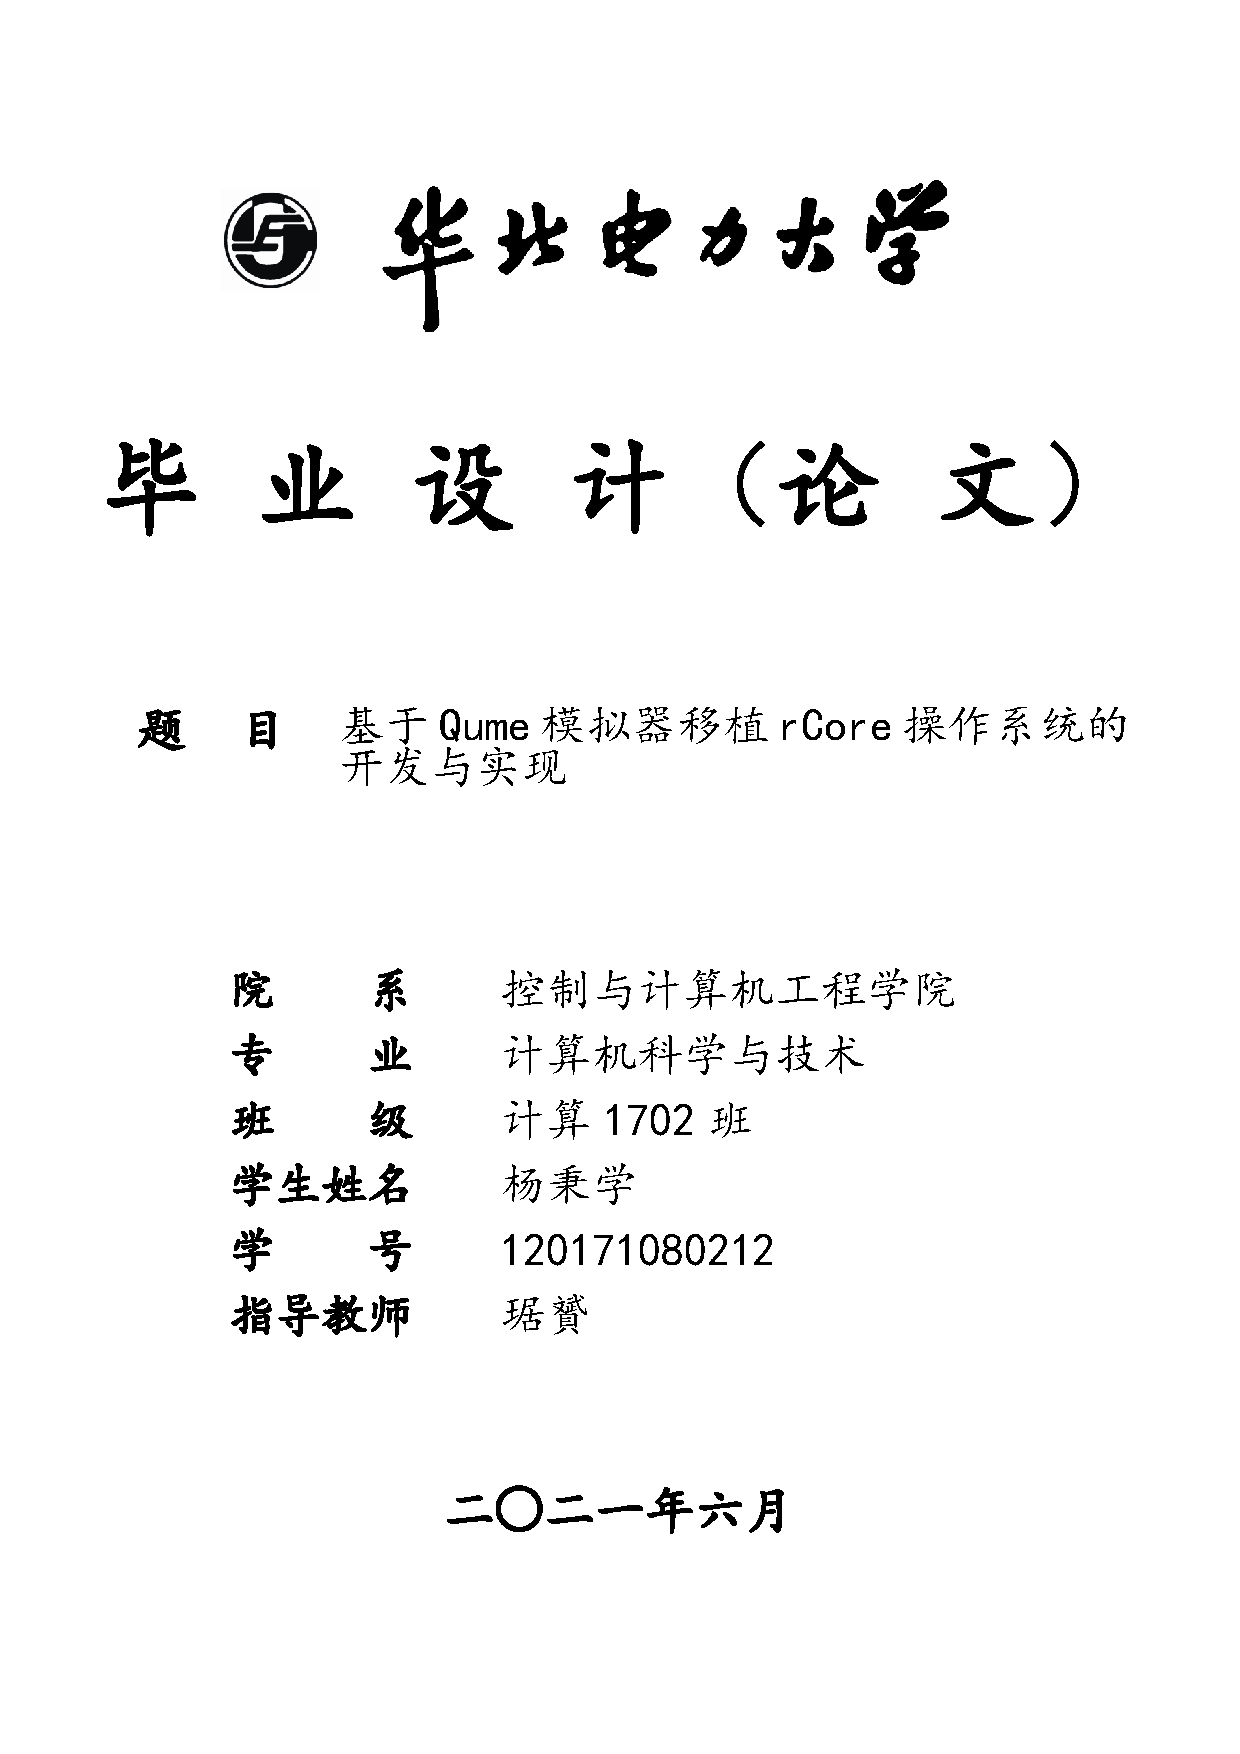
\includepdf[pages={1}]{part/cover.pdf}
%% 这是封面
\begin{flushright}
\end{flushright}
\begin{center}
    \vskip 1.5cm
    
\includegraphics[scale=0.6]{figs/ncepu.eps}%学校图标
\end{center}
\begin{center}
    \vskip 1.5cm
    
\includegraphics[scale=0.6]{figs/bthesistitle.eps}%毕业设计图标
\end{center}
\begin{center}
  \vskip 2cm
    \fontsize{15}{1} \textbf{题目} {基于Qemu模拟器移植rCore操作系统的开发与实现}
  \vskip 2.5cm
\end{center}

\begin{center}
\begin{table}[]
\begin{tabular}{ll}
院\quad\quad 系 & 控制与计算机工程学院 \\
专\quad\quad 业 & 计算机科学与技术 \\
班\quad\quad 级 & 计算1702班 \\
学生姓名 & 杨秉学 \\
学\quad\quad 号 & 120171080212 \\
指导教师 & 琚贇 
\end{tabular}
\end{table}
\end{center}

% \begin{center}
%   \begin{tabular}{l}
% 
%     院\quad\quad 系 \underline{\qquad 控制与计算机工程学院 \quad }\\\\
%     专\quad\quad 业 \underline{\qquad 计算机科学与技术 \quad\qquad}\\\\
%     % \quad 代表空格,输入题目后自己调长度
%     班\quad\quad 级 \underline{\qquad\quad 计算1702班 \quad\qquad\quad }\\\\
%     学生姓名 \underline{\qquad\qquad 杨秉学\qquad\qquad\qquad}\\\\
%     学\quad\quad 号 \underline{\qquad\quad 120171080212 \qquad\qquad }\\\\
%     指导教师 \underline{\qquad\qquad\quad 琚贇\qquad\qquad\qquad }\\\\
% 
%   \end{tabular}
% \end{center}
\begin{center}
        \vskip 2.5cm
    {2021} 年{\quad 六\quad }月{\qquad \qquad }日

\end{center}
\thispagestyle{empty} %去除本页页码

%--------------------------------------------------------------------------------
%%摘要
%%%% 中文摘要
% 这是中文摘要
\newpage
\pagenumbering{Roman}
\renewcommand{\abstractname}{\heiti{\Large{摘\ \ \ \ 要}}}
\begin{abstract}
%%%%%%%%%%%%%%%%%%%%%%%%
%想把一些非章节的部分加入目录
\phantomsection
\addcontentsline{toc}{section}{\heiti{\Large{摘 \quad \quad 要}}}    
%%%%%%%%%%%%%%%%%%%%%%%%
~\\
{\large{
    \indent
    RISC-V是一款近年来最为流行的开源指令集架构,而且被广泛应用于各个场景。

    本文是采用Qemu虚拟化模拟仿真出RISC-V指令环境,用于解决跨平台的模型部署和运行问题。并在模拟出来的RISC-V处理器上面进行移植Linux内核、文件系统以及网络协议栈,最后尝试在上面运行RISC-V程序,主要目的是因为本科所学知识理论与实践衔接并不紧密,感觉“纸上得来终觉浅,绝知此事要躬行”,很多内容似懂非懂,一方面还能凭借书本的记忆说上几句,做对几道题,回答上老师的几个问题;另一方面心里又十分清楚地认识到自己学得不是很到位,很多知识内容如果稍微较真一点深入地探讨一下,就会发现自己有很多内容解释不清楚,更谈不上熟练驾驭了,所以本文将对本科所学有关操作系统,计算机组成原理,计算机体系结构还有计算机网络等计算机科学核心课程内容结合RISC-V 指令集和 Linux 操作系统的移植包括一步步完善基本功能来达到对知识的综合理解与回顾。}}


% 下面的是400字,心里比较一下    {\large{正文部分包括:前言、论文主体和结论。要求文章结构严谨,语言流畅,内容正确。前言作为论文的开场白,要以简短的篇幅,说明毕业设计(论文)工作的选题目的和意义、国内外文献综述(或研究动态)以及论文所要研究的正文部分包括:前言、论文主体和结论。要求文章结构严谨,语言流畅,内容正确。前言作为论文的开场白,要以简短的篇幅,说明毕业设计(论文)工作的选题目的和意义、国内外文献综述(或研究动态)以及论文所要研究的正文部分包括:前言、论文主体和结论。要求文章结构严谨,语言流畅,内容正确。前言作为论文的开场白,要以简短的篇幅,说明毕业设计(论文)工作的选题目的和意义、国内外文献综述(或研究动态)以及论文所要研究的正文部分包括:前言、论文主体和结论。要求文章结构严谨,语言流畅,内容正确。前言作为论文的开场白,要以简短的篇幅,说明毕业设计(论文)工作的选题目的和意义、国内外文献综述(或研究动态)以及论文所要研究的}}

%\\ \hspace*{\fill} \\  %换行,用空格填充,再换行,即可实现空出一整行的效果,不需任何环境调整
~\\
\noindent %取消首航缩进
    {\large{\textbf{关键字}:RISC-V,Qemu,linux}}
\end{abstract}

%%%% 英文摘要
% 这是英文摘要
\newpage
\renewcommand{\abstractname}{\Large \textbf{ABSTRACT}}
\begin{abstract}
\phantomsection    
\addcontentsline{toc}{section}{\heiti{\Large{ABSTRACT}}}    

~\\
{\large{
    \indent
    RISC - V is one of the most popular open source instruction set architecture in recent years, and is widely used in various application scenarios. 

This paper uses Virtualization Technology of QEMU to simulate RISC-V instruction environment, which is used to solve the problem of cross-platform model        deployment and operation.In addition, I transplanted Linux kernel, file system and network protocol stack on the simulated RISC-V processor, and finally tried to run RISC- V program on it. The main purpose was that there was not relative combination of theory and practice of the knowledge that I had learned in the undergraduate course. As the old saying goes "Paper will sleep shallow, never know the matter want to practice." On the one hand, can also rely on the memory of the book to say a few words, do a few questions, answer the teacher's several questions; On the other hand, I clearly realize that I have not learned well. If I study up on it a little more deeply, I will find that I can't explain a lot of concept clearly, let alone master it skillfully. Therefore, this paper will refer to the operating system, principle of computer organization, Computer architecture and computer networking that are the core   courses of computer science, incorporating RISC-V instruction set and Linux operating system, including step by step improvement of basic functions to achieve  a comprehensive understanding of the knowledge.

    }}

~\\
\noindent %取消首航缩进
    {\large \textbf{KEY WORDS:}RISC-V, Qemu,linux}
\end{abstract}

%--------------------------------------------------------------------------------
%% 目录
\newpage
\tableofcontents
\thispagestyle{empty}
%--------------------------------------------------------------------------------
%% 章节样式
\newpage
\pagenumbering{arabic} %页码是阿拉伯数字
% 本章节是介绍项目的背景信息
\section{绪论}
\subsection{课题研究背景和意义}
在“中兴事件”刚过没多久,某些国家就开始发动“华为事件”,进行各种制裁,这对我国半导体产业的打击极大,是可忍孰不可忍,放眼整个产业链,我们国家连一个像样的成熟指令集架构都没有,连一个可大规模商用的操作系统都没有,当我们想研究开发产品竟然还需要看别人脸色来得到授权,这是莫大的耻辱。为什么外国人能做出来,我们就做不出来,我们也并不比他们差什么。所以,我觉得我有必要研究这样的问题了,这就是为什么我毕业设计要研究操作系统,指令集这样的内容,帝国主义封锁我们,不让我们发展,但我偏偏就要研究这些偏底层的原理。

首先是选择的指令集——Risc-v,它是一个最近流行基于RISC的指令集架构,它就类似于软件领域开源的linux一样,Risc-V也有在很多领域发挥作用,如果将linux与RiSC-V结合一起来发展的话,我们就可以利用已有的生态,站在巨人们的肩膀上完成自己的目标,而且开源的话可以集思广益,大家一起参与进来,在这个过程中可以发现自己的不足,然后改正,这本身就是一个学习提升的过程,是一个充满意义的事情。


\subsection{国内外研究现状}
美国的加州大学伯克利分校是最早开始RISC-V的开发,并且经过多次优化完善最终形成的第5代精简指令集(RISC),并于2014年发布,它集百家之长吸收了ARM,MIPS,x86和PowerPC的丰富经验,是一个经过模块化的可扩展可以面对不同的应用场景的指令集,它可以通过组合他的不同模块满足不同需求,而且像ARM的传统指令集是不可以进行指令集扩展的,
RISC-V是支持指令扩展的,最关键的还是RISC-V指令架构是没有历史包袱的,
具体体现在以下几个方面,
1.手册页数比较少,与x86和ARM架构的手册达到几千页的数量不同RISC-V架构的手册也就区区不到三百页;2.指令数目上,不同于x86和ARM的指令数那么多并且繁杂,在加上由于历史原因他们不同架构之间的不同分支也相互彼此不兼容。
而RISC-V没有历史包袱,在设计指令集的时候重新从头开始设计,
最终只包含40多个基础指令,并根据这些做为公共部分,再扩展出其他常用的模块指令。实现起来比较简单,在硬件平台上实现也不是很难。

虽然我们的学校的确与美帝之间存在差距,但是这都不算什么,因为就算他们现在比我们发展要超前也这不代表以后永远都会领先我们,如果我们把精力,资源放在这方面,假以时日我们是会迎头赶上的,也可以做出属于自己的产业链。

目前国外SiFive公司服务做的不错,主要业务是提供商业化的针对RISC-V指令集架构设计的应用处理器的IP、相关配套的软件开发平台以及与芯片相关的多种应对策略。
SiFive在2018年注册独立公司SaiFan在中国运行,来服务于中国市场为客服提供服务;
另一家国外公司——Green WavesIoT ,该公司主营功耗低基于RISC-V的用于边缘应用的IP和处理器\cite{Risc-V_development}。

我们之前说了很多关于真正实现国产化指令集的设想,现在RISC-V指令集架构就是这样的一个机遇。
以前的国产芯片领域的开发基本上都需要得到国外公司的授权的才能开发,典型的就是ARM架构,我们的发展花费了大约有十几年的时间来壮大,但重要的是,这些指令集架构是属于外国公司,并不是免费白让我们使用,从根本上来讲是需要他们这些大公司来允许我们使用,如果我国以后使用RISC-V的话,
一方面是可以省去把用来给外国公司交的授权费,用来放在更好的科研攻关上面;
另一方面,外国企业可以随时完全停止合作授权的时代一去不复返了。相比较我们民族大力发展来让自己实现一套自主的指令集架构,成本高,技术难度大,所以这件事本身又没有太大的经济技术应用价值,
因为开发出来一个处理器是要在整个世界上流通的,这样才有可能让各地的软件生态加入建设中来。所以RISC-V的横空出现,就可以很好的处理相应的关系。

国内的芯来科技模仿SiFive做的也不错,提供多个RISC-V IP, 并同时提供蜂鸟E203开发板; 
位于中国台湾的公司——Andes Technology同样推出基于RISC-V的芯片产品; 
在2018年4月,阿里的平头哥收购了中天微并展开了自己的研究,并在2021年发布了目前世界范围内性能最优的RISC-V芯片玄铁910,并且可以与Android OS衔接完美,
这表明目前完善的Android生态环境可以运行在国产RISC-V芯片上了,换句话说软件的生态已经基本解决了。

最后RISC-V对IoT的发展也同样巨大,
现在碎片化是物联网和边缘计算的发展表象,而且以应用为核心的发展方向也逐步成为发展趋势,不同以往传统的围绕着芯片,因为这样的发展方式就会导致以发展模组和应用的公司为核心的,而替代了从前那种以芯片公司为核心的发展方式,传统方式已经面对如今的发展趋势表现出力不从心了。
我们以ARM为例,其特点是不仅价格不亲民每次发布还挺长时间的,如果用于物联网相同的使用场景,就会在市场上趋近相同的的竞争,加上成本高等因素,导致大家都不原意去开发,最终除了少数大企业才能最早买到IP,其他公司只能望尘莫及,这样的后果就是ARM的发展很难去高效的来应对碎片化应用需求。

\subsection{本文研究内容}
本文主要参考孙卫真,刘雪松,朱威浦和向勇老师的《基于RISC-V的计算机系统综合实验设计》\cite{基于RISC-V的计算机系统综合实验设计}上面的内容在Qemu模拟器上将linux试图移植到RISC-V的平台上面,并逐步实现实验环境的搭建,交叉工具链的编译,完善文件系统,安装网络协议栈等现代操作系统应该具备的基本功能,并解决在此过程中遇到的种种挑战,种种报错以及解决方案,最后运行一个RISC-V指令集的简单程序验证一下是否移植成功。

虽然,已经国内已经有人做出了基于RISC-V处理器内核,linus也把riscv-linux合并到Linux的主分支上了,但是我这个毕设的内容就是自己想进行一遍,是验证性的实验,虽然我也知道我现在做的这些事情看来有些微不足道,但是我想既然我已经努力开始做了,就已经具有了加速度,根据$v= v_{0} + at $让子弹再飞一会儿,最终就会获得丰收的成绩。



\newpage  % 课题研究背景和意义
% 本章节是介绍 RISC-V的
\section{计算机组成与设计——基于RISC-V}
本章节是根据 David A. Patterson 的著作\cite{Computer_Organization_and_Design_riscv}以及浙江大学刘鹏博导的公开课\cite{Computer_Organization_and_Design_ZJU}来改编实现的。

\subsection{指令表示方法与指令格式}
如果把计算机比作一个在说话的人,那么指令就是每一个单词,指令集就是全部词汇所构成的词汇表

\subsubsection{R指令}
\textbf{R指令}是用于寄存器与寄存器之间算数运算的

一条R型指令的格式划分如图\ref{fig:R-Format_Instruction_Layout}所示,R型指令可以划分为6个域,其中31-25这7bit宽的是功能码7,24-20这5为是源寄存器2,19-15这5为是源寄存器1,14-12这3bit宽的是功能码3,11-7这5bit宽的目的寄存器rd,6-0这7位宽的操作码(部分规定了该指令是什么指令)。

\begin{figure}[htbp]
  \centering %居中显示
  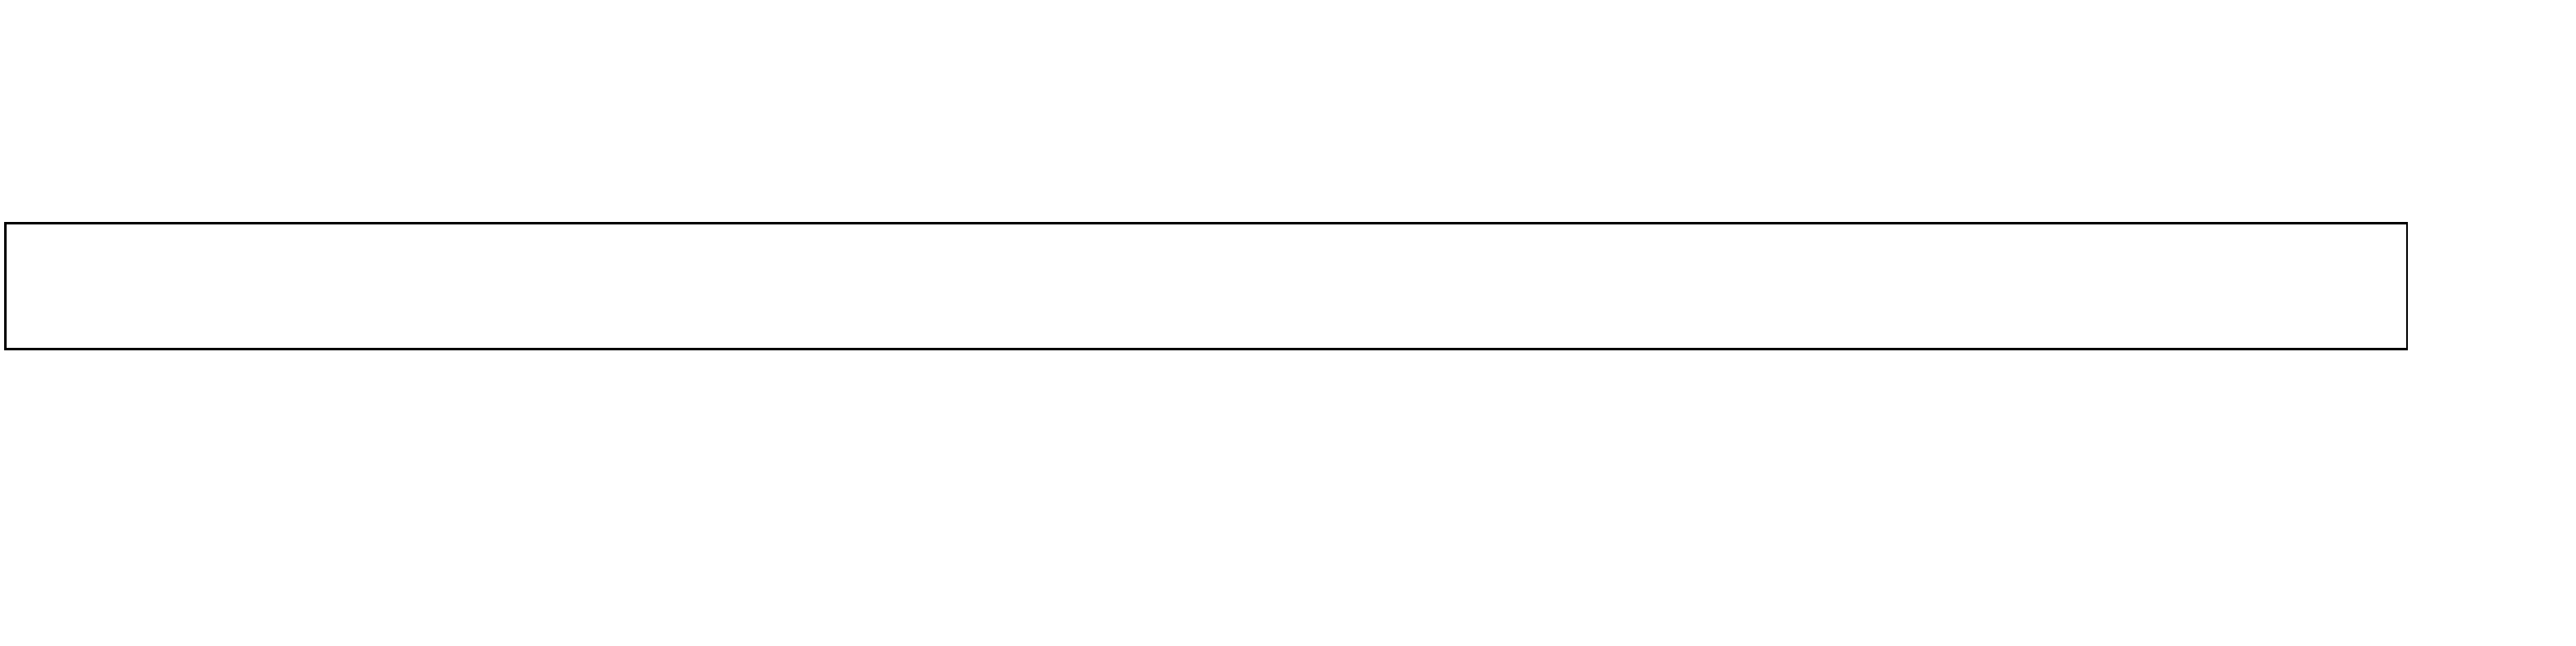
\includegraphics[width=0.8 \textwidth]{figs/RISC-V/指令表示/R-Format_Instruction_Layout.eps}
  \caption{R型指令格式的划分\\ 其中每个域中的文字表示该域的名称;域上的数字表示,该域的起始与终止位置;每个域下面的数字,表示每个域所占据的bit位数}
  \label{fig:R-Format_Instruction_Layout} %设置图形引用名称
\end{figure}
所有R指令的opcode部分都是2进制数:0110011,funct7与funct3是和opcode结合起来一起使用的,三者组合一起规定指令的操作。

rs1,rs2是源寄存器(Source Rggister),用于存放操作数的源地址的,rd是目的寄存器(Destination Rggister),指定接收结果值的寄存器编号,这三个寄存器都存放5位无符号整数(对应十进制$2^5=32$),对应0˜31的通用寄存器中的其中一个。


\subsubsection{I指令}
\textbf{I指令}是用于寄存器与立即数之间算数运算和读取的 

其实如果是我自己设计指令架构,我很有可能将操作寄存器,操作数用一个指令全部实现,但是有一个问题,就是指令中的位长,比方说R指令的源地址和目的地址才5bit,最多就能表示10进制的32位,那要是操作数字就显得有些有限;但是如果你把指令中的位长加长的话,就会造成可以表示的10进制数太多,但是寄存器就32了,造成不必要的浪费。

所以,I型指令可以在R型指令的基础上做一些稍微的改动即可,如图\ref{fig:R_I}所示。

\begin{figure}[htbp]
  \centering %居中显示
  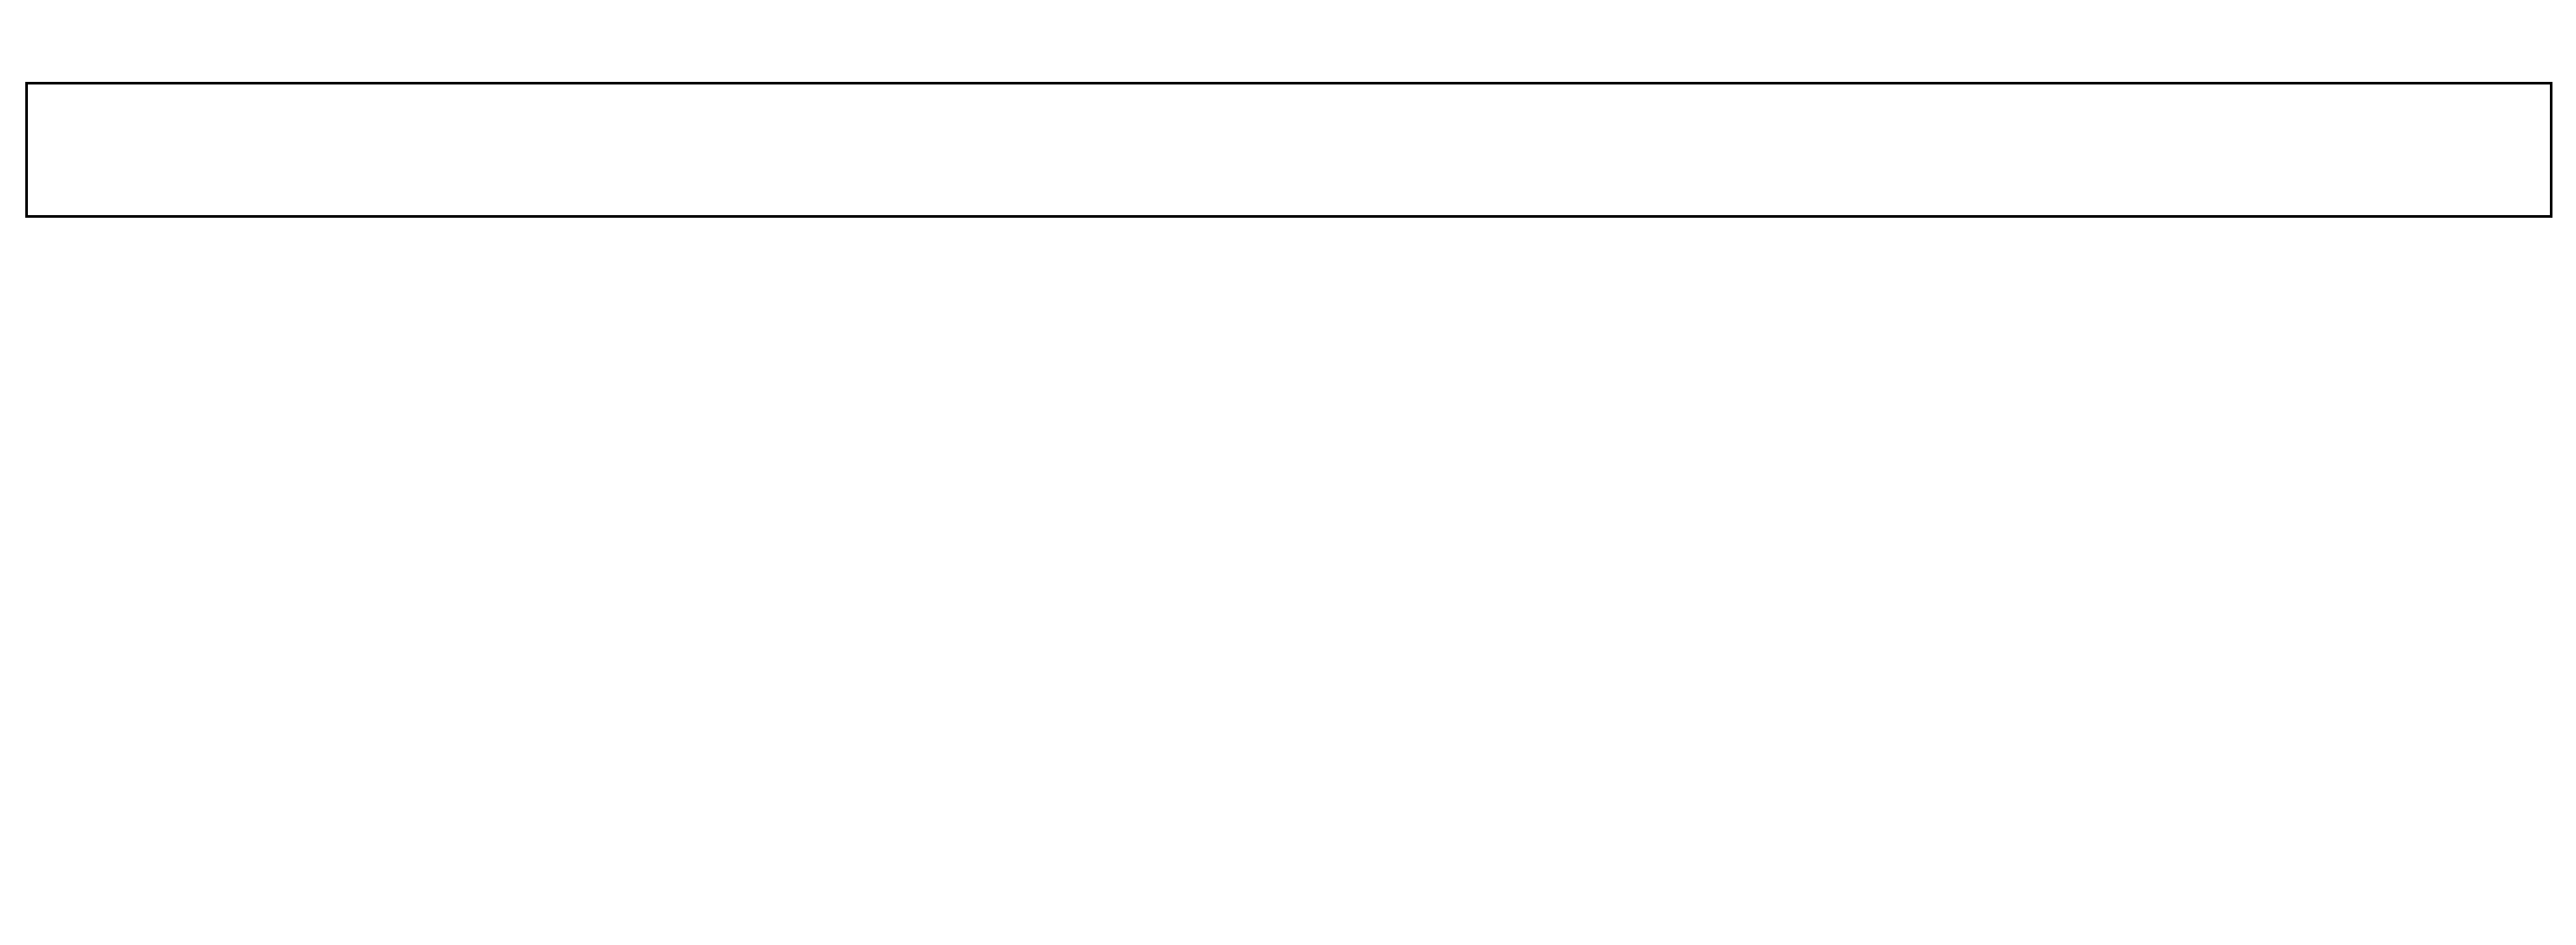
\includegraphics[width=0.8 \textwidth]{figs/RISC-V/指令表示/R_I.eps}
  \caption{I型指令就是把R型指令的前两个域合并成一个了12位的有符号数}
  \label{fig:R_I} %设置图形引用名称
\end{figure}



\subsubsection{S指令}
用于写存储器的

\subsubsection{B指令}
用于分支转移操作的,其实是S指令的一个变体,之前也叫\textbf{SB指令}

\subsubsection{U指令}
用于高20-bit位立即数操作

\subsubsection{J指令}
用于跳转操作,其实是U指令的一个变体,之前也叫\textbf{UJ指令}


\subsection{流水线}
\subsubsection{处理器性能度量方法}
首先,我认为在我们研究之前应该明确我们常说的提高性能是指什么,是表示更快的响应时间?从而更快的完成需要执行的任务?还是单位时间内能完成更多的任务?还是使用寿命更长一些?

我觉得性能的本质是——

\begin{equation}\label{eq:Computer_Analogy}
    \frac{ Time }{ Program } = \frac{ Instructions }{ Program } * \frac{ Cycles }{ Instruction } * \frac{ Time }{ Cycle }
\end{equation}

公式 (\ref{eq:Computer_Analogy})是与处理器性能有关的定理

\subsubsection{流水线的设计}
处理器执行一条指令的步骤——取指,译码,执行,访存,写回。

\subsubsection{结构冒险}
造成这个冒险的原因是硬件不支持同一周期执行多条指令

这个也比较好解决1.让其他阻塞一下等待硬件空闲下来在使用,2.要么就是多添加点硬件。



\subsubsection{数据冒险}
导致数据冒险发生简言之就是不同指令之间存在数据的关联,造成了无法提供指令执行所需的数据,进而指令不能在预期的时钟周期内执行。

解决方案就是 1.让其他阻塞一下等待数据使用完在使用,2.增加一个\textbf{旁路(bypassing)},这样的好处就是不需要等待指令完成就可以超市解决数据冒险。如图\ref{fig:Data_Hazards1} 所示,第一条add指令执行EX阶段的输出前递到sub指令的EX阶段的输入,替换sub指令在第二阶段督促的寄存器X1的值。

\begin{figure}[htbp]
  \centering %居中显示
  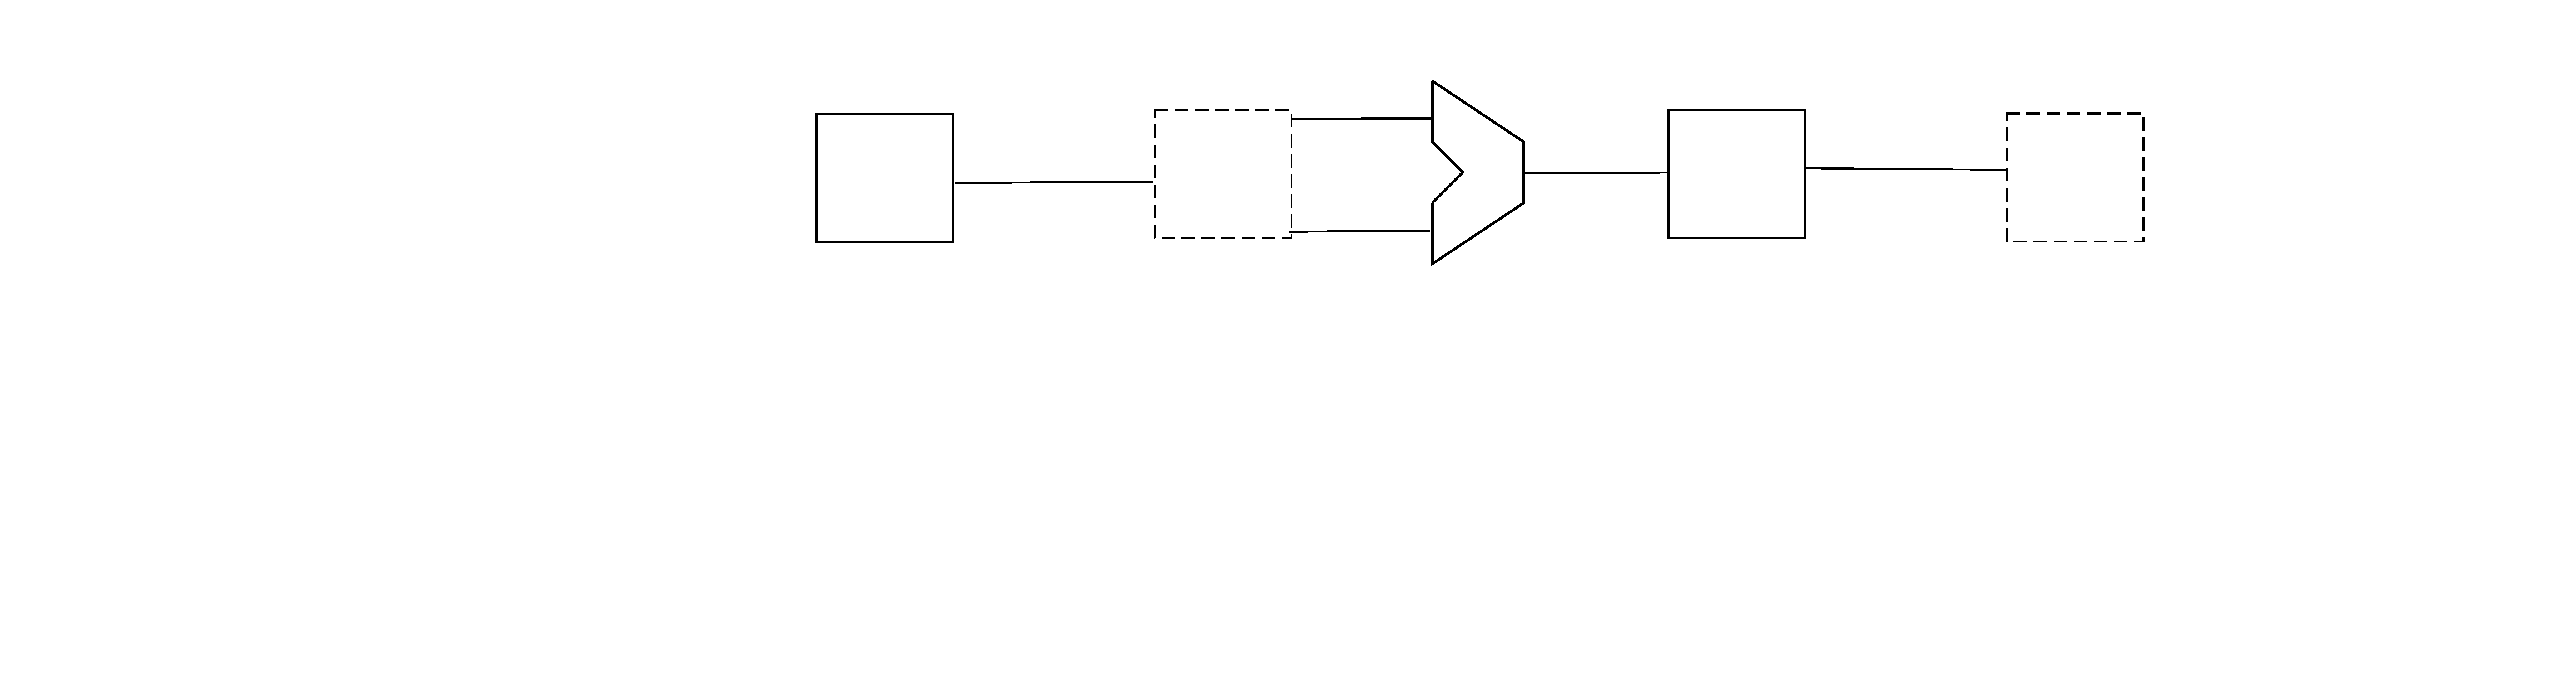
\includegraphics[width=0.8 \textwidth]{figs/RISC-V/流水线/数据冒险1.eps}
  \caption{这张图片就显示了旁路的效果}
  \label{fig:Data_Hazards1} %设置图形引用名称
\end{figure}

但是有时尽管使用了旁路,也不可避免的需要\textbf{流水线停顿(pipeline Stall)},俗称\textbf{气泡(bubble)},图\ref{fig:Data_Hazards2}就是load指令执行之后,紧跟着一条需要使用他结果的R型指令

\begin{figure}[htbp]
  \centering %居中显示
  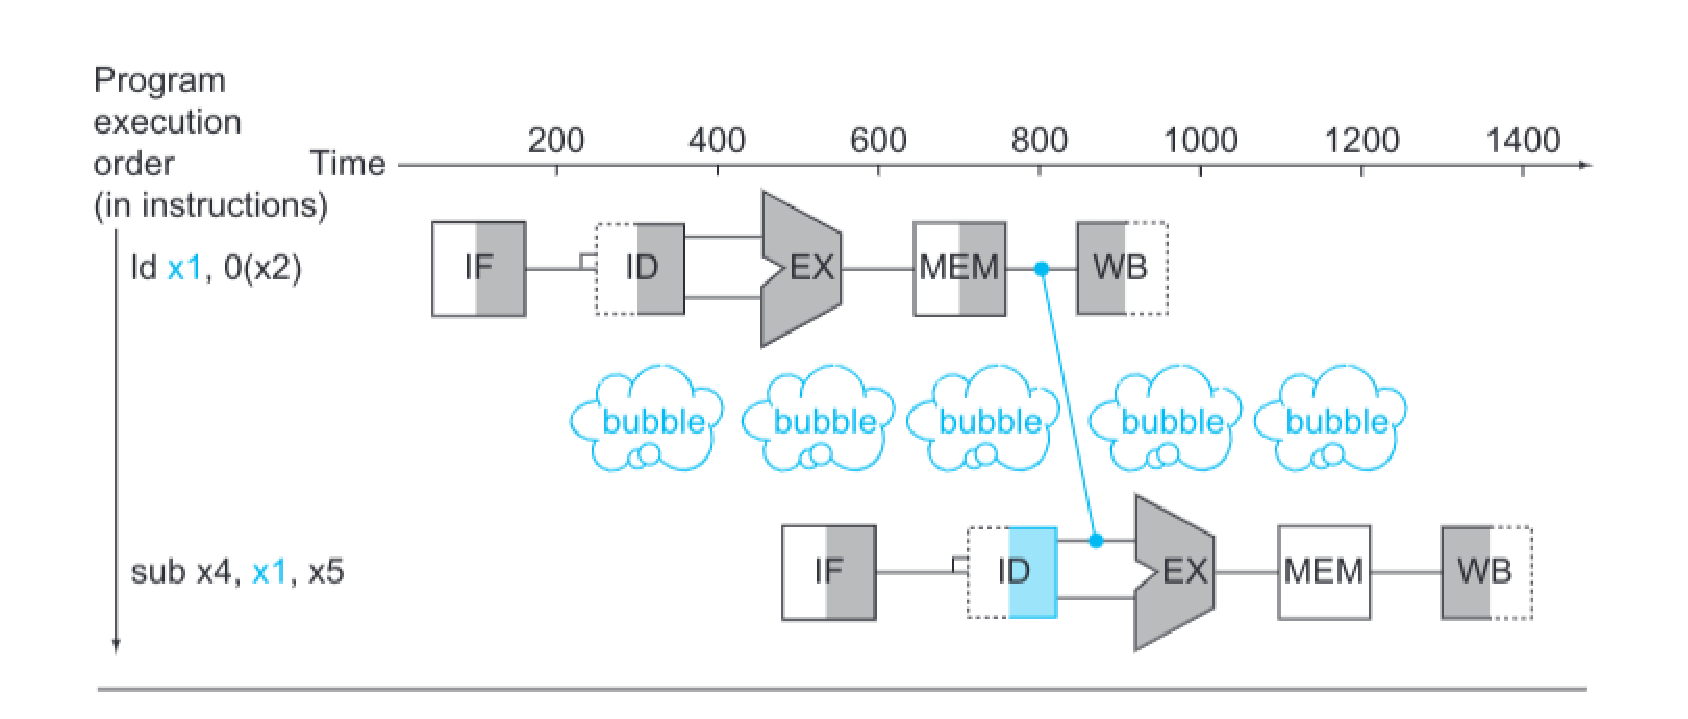
\includegraphics[width=0.8 \textwidth]{figs/RISC-V/流水线/数据冒险2.eps}
  \caption{这张就表示有时即使使用旁路,也许要阻塞等待}
  \label{fig:Data_Hazards2} %设置图形引用名称
\end{figure}


\subsubsection{控制冒险}
这种冒险发生在根据一条指令的结果判断接下来要执行的分支程序。如图\ref{fig:Control_Hazards}所示

\begin{figure}[htbp]
  \centering %居中显示
  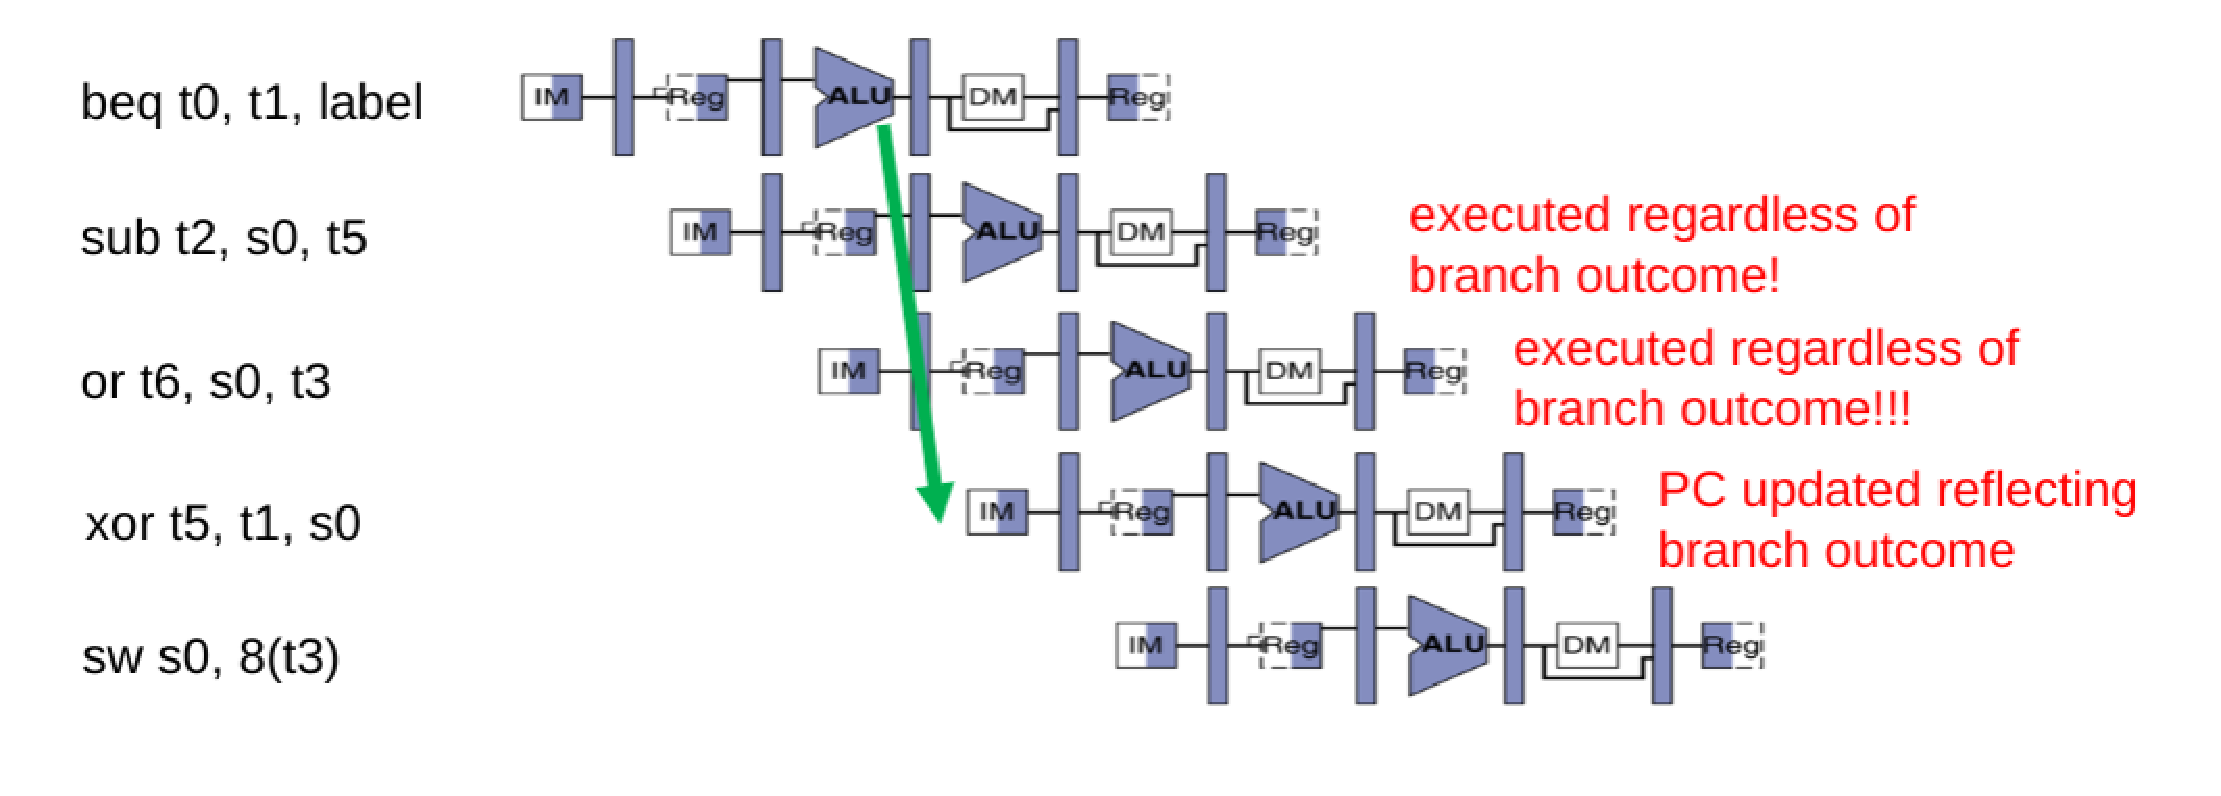
\includegraphics[width=0.8 \textwidth]{figs/RISC-V/流水线/控制冒险.eps}
  \caption{控制冒险}
  \label{fig:Control_Hazards} %设置图形引用名称
\end{figure}

解决方法1.阻塞等待,2.采用\textbf{分支预测},要是预测对了,就继续执行,如图\ref{fig:Control_Hazards_Success};如果预测错了,流水线清空刚才加载错误的指令,重新在装载正确的指令,如图\ref{fig:Control_Hazards_Fail}。

\begin{figure}[htbp]
  \centering %居中显示
  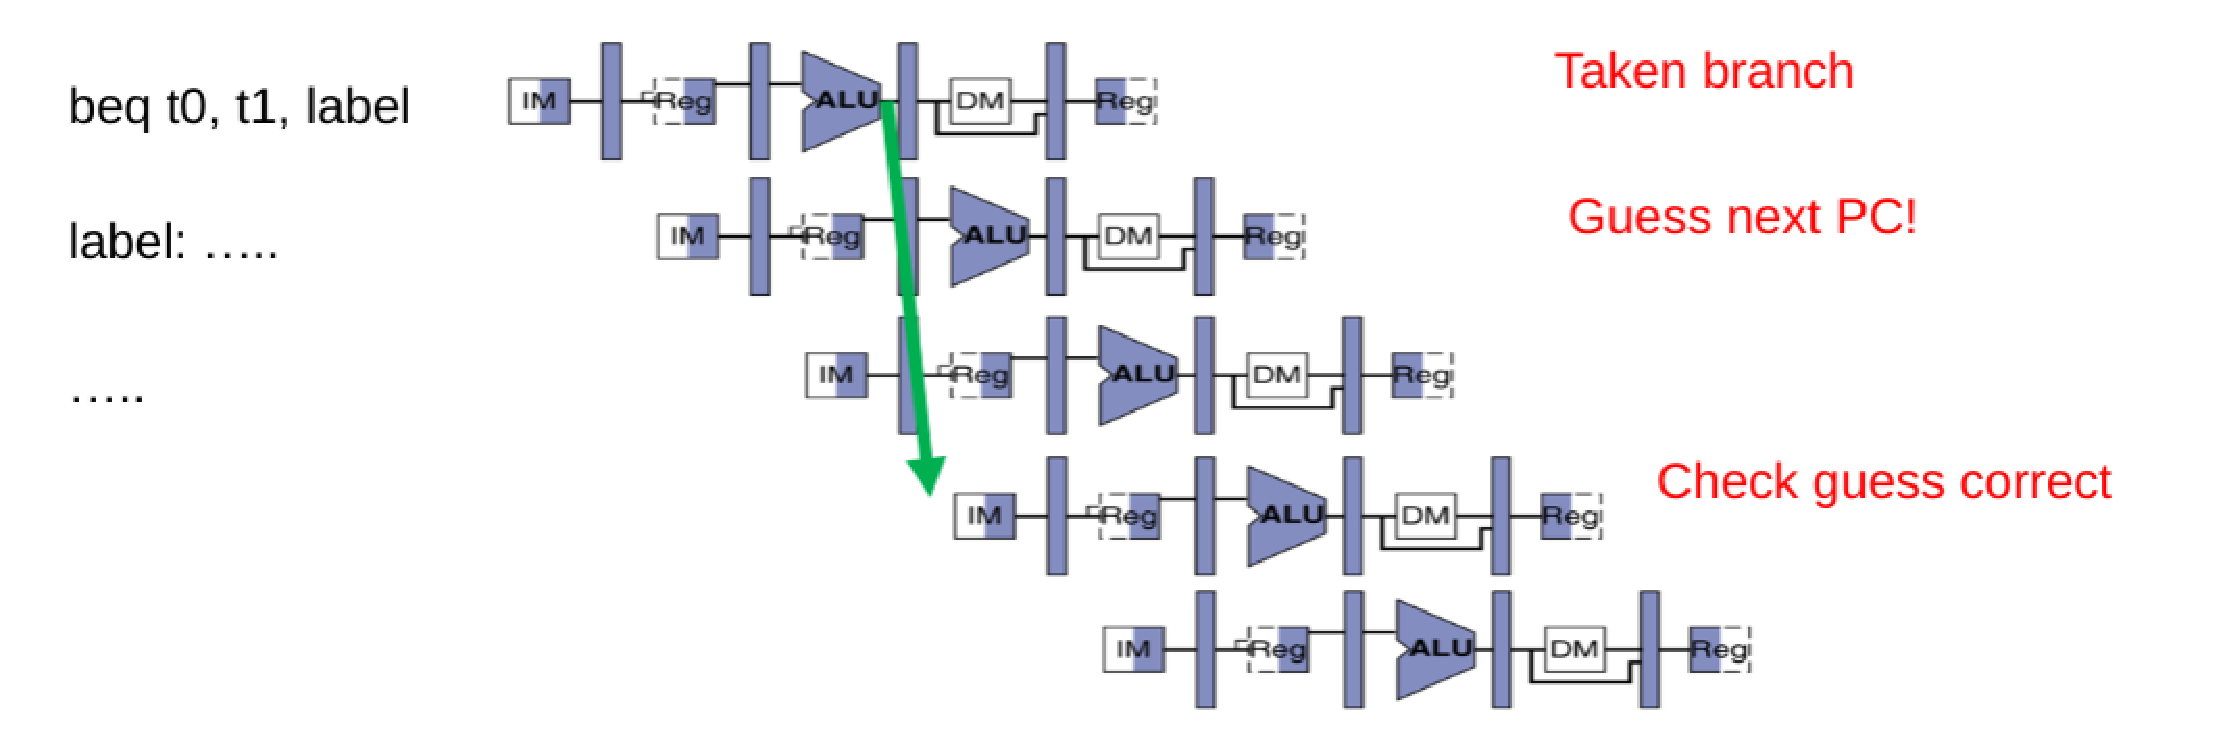
\includegraphics[width=0.8 \textwidth]{figs/RISC-V/流水线/控制冒险_预测成功.eps}
  \caption{分支预测:预测成功}
  \label{fig:Control_Hazards_Success} %设置图形引用名称
\end{figure}

\begin{figure}[htbp]
  \centering %居中显示
  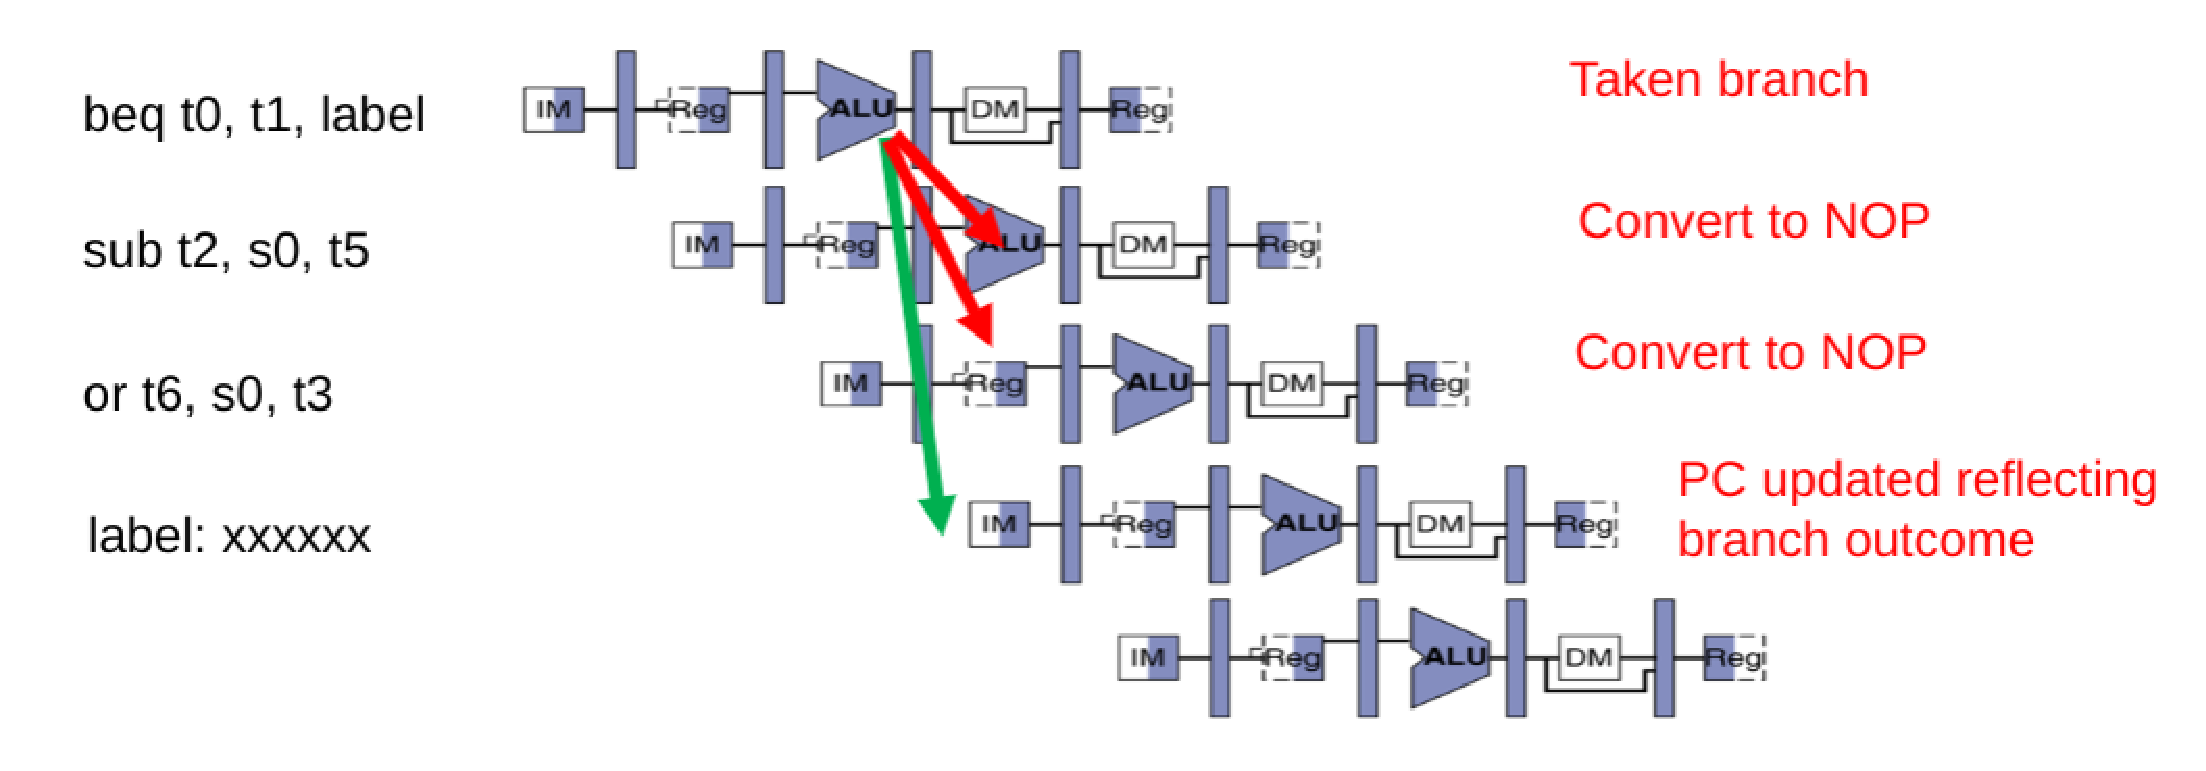
\includegraphics[width=0.8 \textwidth]{figs/RISC-V/流水线/控制冒险_预测失败.eps}
  \caption{分支预测:预测失败}
  \label{fig:Control_Hazards_Fail} %设置图形引用名称
\end{figure}







\newpage % 介绍RISC-V架构内容
% 本章节介绍Qemu的原理
\section{Qemu \& KVM 基本原理}
\subsection{虚拟化}
在维基百科中虚拟化的解释为:“In computing,virtualization refers to the act of creating a virtual(rather than actual)version of something,including virtual computer hardware platforms,storage devices,and computer network resources。”\cite{Wikipedia_Virtualization}, 
简单来说,计算机模拟出一个虚拟并不存在的(而非实际)计算机实体就是虚拟化,其中包括虚拟出来的计算机硬件平台、存储设备,以及网络资源。
由此可见,虚拟化技术是一种将硬件资源(如处理器、Memory、storage、NetWork resource etc)提取出来,最终成为一个虚拟的资源池,并对其提供分割、重新组合的操作,以达到资源利用最大化。

\subsubsection{软件虚拟化}
本文所介绍的是使用Qemu来实现VMM层,即仅使用软件实现的方式来运行客户机要执行的指令。
Qemu工作方式是在软件层面实现对指令的二进制翻译,简单来说就是Qemu是一个翻译官,它将使用某套指令集的二进制编码翻译成基于另一套指令集的编码并最终输出到最终架构下的代码交给客户机,QEMU会拦截每一条客户机执行的指令,并转换成宿主机处理器架构的指令,
最后由宿主机的物理硬件来执行相应的指令,由此往复完成虚拟化的实现。

\subsubsection{硬件虚拟化}
这里以通用的x86体系结构为例,Intel在2005年就加入硬件虚拟化的支持——Intel VT。
这也就以为着硬件平台本身支持客户机与宿主机指令间相互转换并执行,而不再像以前那样需要VMM截获重定向这种软件实现方式。

其实我们通过纯粹用软件中的模块管理层面上直接对管理整个客户机服务的进程就是通过要在整个linux上的一个内部物理执行进程,
客户机正常执行访存操作时,实际上我们就是通过Linux上对内核管理的虚拟内存,以前是使用linux中的内核软件来实现GVA(客户机虚拟地址)到GPA(客户机物理地址)再到HVA(宿主机虚拟地址),最后到HPA(宿主机物理地址)的这四步的转换,这个机制也称为“影子页表”。
但是原本就是访问一个地址很简单的操作却大费周折要经过四步执行,对于计算机来说,这样的代价特别大,所以后来这种靠软件实现的方式逐步被硬件逻辑取代,这种硬件逻辑就是Intel的EPT技术(或者AMD的NPT技术),靠硬件自动算出GPA到HPA的过程,转换的过程一步到位。

\subsection{硬件虚拟化介绍}

\subsubsection{CPU虚拟化}
根据上文的介绍,软件实现虚拟化的成本代价比较大,所以像Intel这样的硬件厂商慢慢地在硬件层面上实现虚拟化。

关键技术——VMX(virtual-machine extensions),
这项技术就是Intel在处理器层面上提供了对实现虚拟化在技术上的支持。
根据查询Intel的官方文档\cite{Intel_VMX}可知 VMX有两种操作模式:VMX根操作(root operation)与VMX非根操作(non-root operation)。

简单的区分,在VMX根操作模式运行KVM下,而VMX非根模式下运行的是整个运行在虚拟机中的客户机完整的软件栈(包括操作系统和应用程序)。VMX根操作模式与非VMX模式之间是可以相互转化的,当从VMX跟模式进入VMX 非根操作模式被称为“VM Entry”;从VMX非根操作模式退出到VMX根操作模式,被称为“VM Exit”。

可能都是Intel发明的缘故,VMX的根操作模式与非VMX模式像极了x86处理器的各种执行模式,
区别只是VMX的根操作现在已经支持了新的VMX相关的指令集以及一些对相关控制寄存器的操作。
而由于VMX的非根操作模式是一个相对受限的执行环境,为了更好地适应在虚拟化中的变化而专门进行了一定的修改;
VMX的根操作模式与非VMX模式之间的转换如同处理器的各种门的特权集转换一样,当客户机中执行的一些特殊的敏感指令或者一些异常会触发“VM Exit”退到虚拟机监控器中,从而运行在VMX根模式。这样的行为看似很麻烦,但是也正是因为这样的限制,才让虚拟机监控器保持了对处理器资源的更好的控制。

为了更好的理解,VMM 与 Guest 之间 以及VMX的根操作模式与非根操作模式是如何转换的,
交互一个虚拟机监控器软件的最基础的运行生命周期及其与客户机的交互如图 \ref{fig:VMM_Guest} 所示。
软件想进入VMM操作模式,需要通过执行VMXON指令才能进入;当已经进入VMM模式以后,想在进入客户机执行模式,即VMX非根模式,需要通过执行VMLAUNCH和VMRESUME指令进入;
当在VMX非根模式下触发VM Exit时,处理器执行控制权会再次回到宿主机的虚拟机监控器上;
最后虚拟机监控可以通过执行VMXOFF指令退出VMX执行模式。

\begin{figure}[htbp]
    \centering
    \def\svgwidth{\columnwidth}
    \import{./figs/RISC-V/KVM/VMM_Guest/}{VMM_Guest.pdf_tex}
    \caption{VMM与Guest之间的交互}
    \label{fig:VMM_Guest}
\end{figure}


如图\ref{fig:VMM_Guest} 中需要完成的转换过程,
在该过程中是通过使用VMCS(virtual-machinecontrol data structure)的数据结构来实现逻辑处理器完成根模式和非根模式之间的切换的;
而处理器是通过使用VMCS指针来进行访问VMCS结构的,并对其进行操作。
其实VMCS指针其实也没什么神奇的,本质上就是一个指向VMCS结构的64位的地址,可以通过使用VMPTRST和VMPTRLD指令对VMCS指针进行读写,使用MREAD、VMWRITE和VMCLEAR等指令对VMCS实现配置。

对于一个逻辑处理器,表面上看它是可以一起维护多个VMCS数据结构,但是具体到某一时刻的时候,就只有一个VMCS在当前真正生效。多个VMCS之间也是可以相互切换的,VMPTRLD指令就让某个VMCS在当前生效,而其他VMCS就自然成为不是当前生效的。一个虚拟机监控器会为一个虚拟客户机上的每一个逻辑处理器维护一个VMCS数据结构。

\subsubsection{内存虚拟化}
内存虚拟化的目的是给虚拟客户机操作系统提供类似实际的物理存储空间——即一个从0地址开始的连续物理内存空间,但是他不仅仅就是提供地址空间,还要同时在多个客户机之间实现隔离和调度。

在虚拟环境下内存地址如图 \ref{fig:Virtual2Physical_Address} 所示。
\begin{figure}[htbp]
    \centering
    \def\svgscale{0.5}
    \import{./figs/RISC-V/KVM/Virtual2Physical_Address/}{Virtual2Physical_Address.pdf_tex}
    \caption{虚拟化环境下的内存地址}
    \label{fig:Virtual2Physical_Address}
\end{figure}

内存虚拟化就是要将客户机虚拟地址(GVA)转化为最终能够访问的宿主机上的物理地址(HPA)。对于客户机操作系统而言,它不可能感知到有内存虚拟化的存在,在应用程序访问虚拟地址时,通过CR3寄存器可以将其转化为物理地址,但是在虚拟化环境中这个物理地址只是客户机的物理地址,还不是真实内存硬件上的物理地址。
所以,虚拟机监控器就非常需要维护从物理客户机虚拟地址映射到客户宿主机上的物理虚拟地址之间的一个动态映射空间关系,
在没有硬件提供的内存虚拟化之前,这个维护映射关系的页表叫作影子页表(Shadow Page Table)。
内存的访问和数据的更新通常是非常频繁的,加之需要一直维护影子页表中的对应关系将会变得非常复杂,开销也较大。同时它还需要为每一个运行的客户机都维护一份影子页表,当客户机数量较多时,其影子页表也会越来越大,占用的内存较大也会是一个问题。

Intel CPU在整个硬件上的设计就引入了EPT(Extended Page Tables,扩展页表),
从而将一个客户机虚拟地址到宿主机物理地址的转换通过硬件来实现。
%首先,通过客户机CR3寄存器将客户机虚拟地址转化为客户机物理地址,然后通过查询EPT来实现客户机物理地址到宿主机物理地址的转化。EPT的控制权在虚拟机监控器中,只有当CPU工作在非根模式时才参与内存地址的转换。使用EPT后,客户机在读写CR3和执行INVLPG指令时不会导致VM Exit,而且客户页表结构自身导致的页故障也不会导致VM Exit。所以通过引入硬件上EPT的支持,简化了内存虚拟化的实现复杂度,同时也提高了内存地址转换的效率。


\subsubsection{I/O虚拟化}
在虚拟化的架构下,虚拟机监控器必须支持来自客户机的I/O请求。通常情况下有以下4种I/O虚拟化方式。

1)设备模拟:在虚拟机监控器中模拟一个传统的I/O设备的特性,比如在QEMU中模拟一个Intel的千兆网卡或者一个IDE硬盘驱动器,在客户机中就暴露为对应的硬件设备。客户机中的I/O请求都由虚拟机监控器捕获并模拟执行后返回给客户机。

2)前后端驱动接口:在虚拟机监控器与客户机之间定义一种全新的适合于虚拟化环境的交互接口,比如常见的virtio协议就是在客户机中暴露为virtio-net、virtio-blk等网络和磁盘设备,在QEMU中实现相应的virtio后端驱动。

3)设备直接分配:将一个物理设备,如一个网卡或硬盘驱动器直接分配给客户机使用,这种情况下I/O请求的链路中很少需要或基本不需要虚拟机监控器的参与,所以性能很好。

4)设备共享分配:其实是设备直接分配方式的一个扩展。在这种模式下,一个(具有特定特性的)物理设备可以支持多个虚拟机功能接口,可以将虚拟功能接口独立地分配给不同的客户机使用。如SR-IOV就是这种方式的一个标准协议。

表\ref{fig:I/O_virtual}展示了这4种I/O虚拟化方式的优缺点,前两种都是纯软件的实现,后两种都需要特定硬件特性的支持。

% 插入表格
\begin{table}[htbp]
     \centering
\begin{tabular}{|c|l|l|}
\hline
\multicolumn{1}{|l|}{} & \textbf{优点}                                                 & \textbf{缺点}                                                                              \\ \hline
设备模拟                   & 兼容性好,不需要额外驱动                                                & \begin{tabular}[c]{@{}l@{}}1.性能较差\\ 2.模拟设备的功能特性支持不够多\end{tabular}                        \\ \hline
前后端接口                  & 性能有所提升                                                      & \begin{tabular}[c]{@{}l@{}}1.兼容性差一些:依赖客户机总安装特定驱动\\ 2.I/O压力大时,后端驱动的CPU资源占用较高\end{tabular} \\ \hline
设备直接分配                 & 性能非常好                                                       & \begin{tabular}[c]{@{}l@{}}1.需要硬件设备的特性支持\\ 2.单个设备只能分配一个客户机\\ 3.很难支持动态迁移\end{tabular}     \\ \hline
设备共享分配                 & \begin{tabular}[c]{@{}l@{}}1.性能非常好\\ 2.单个设备可共享\end{tabular} & \begin{tabular}[c]{@{}l@{}}1.所需设备硬件的特性支持\\ 2.很难支持动态迁移\end{tabular}                       \\ \hline
\end{tabular}
\caption{常见I/O虚拟化方式的优缺点}
\label{fig:I/O_virtual}
\end{table}


\subsection{KVM \& Qemu模拟器介绍}
首先Qemu(Quick Emulator)本身并不完全是KVM的一部分,它是一套由软件模拟实现的。

而KVM(Kernel Virtual Machine)是有两部分组成,一部分是Linux内核的KVM模块,另一块是经过简化后的Qemu。
有了KVM的linux主机将变成一个Hypervisor(虚拟机监控器)。
在x86处理器支持VMX(Virtual Machine Extension)功能以后,
Linux在原有的用户模式和内核模式中又新增加了客户模式,并且客户模式也拥有自己的内核模式和用户模式,其中虚拟机部分就是运行在客户模式中。
三层结构如图\ref{fig:kvm}所示。

\begin{figure}[htbp]
    \centering
    \def\svgscale{0.5}
    \import{./figs/RISC-V/KVM/KVM_3model/}{kvm_3model.pdf_tex}
    \caption{KVM三种模式的层次关系}
    \label{fig:kvm}
\end{figure}    
%『h』当前位置。将图形放置在正文文本中给出该图形环境的地方。如果本页所剩的页面不够,这一参数将不起作用。
%『t』顶部。将图形放置在页面的顶部。
%『b』底部。将图形放置在页面的底部。
%『p』浮动页。将图形放置在一只允许有浮动对象的页面上。

KVM就是在硬件辅助虚拟化技术之上构建起来的虚拟机监控器。

当然,并非要所有这些硬件虚拟化都支持才能运行KVM虚拟化,KVM对硬件最低的依赖是CPU的硬件虚拟化支持。

\subsubsection{KVM内核模块}
KVM模块是KVM虚拟化的核心部分,它在内核是由两部分组成:
其中一个部分是与处理器架构无关的部分,用lsmod命令中可以看到,如图 \ref{fig:lsmod_kvm} 所示,叫作kvm模块;
另一个部分是处理器架构相关的部分,本文是在Intel平台上实验,所以看到的就是 kvm\_intel这个内核模块。
KVM的主要工作就是初始化硬件资源,开启虚拟化模式,将客户机运行在虚拟机模式中,虚拟客户机运行时提供一定的支持。

\begin{figure}[htbp]
  \centering %居中显示
  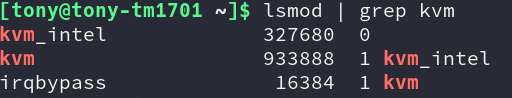
\includegraphics[width=0.9 \textwidth]{figs/RISC-V/KVM/lsmod_kvm.png}
  \caption{lsmod}
  \label{fig:lsmod_kvm} %设置图形引用名称
\end{figure}

以KVM在Intel的x86系列的 CPU上运行为例,在内核加载以后,KVM模块首先会初始化内部的数据结构;
完成一切准备工作以后,KVM模块会继续检测系统当前的CPU,然后打开CPU控制寄存器CR4中的虚拟化模式开关,并通过执行VMXON指令将宿主操作系统(包括KVM模块本身)置于CPU执行模式的虚拟化模式中的根模式;
最后,KVM模块创建特殊设备文件/dev/kvm来等待从用户空间发过来的命令。
接下来,虚拟机的创建和运行将是一个用户空间的应用程序(QEMU)和KVM模块相互配合的过程。

/dev/kvm这个设备文件是一个标准的字符设备,
KVM模块与用户空间QEMU的通信接口主要是一系列针对这个特殊设备文件的loctl调用。
当然,每个虚拟客户机针对/dev/kvm文件的最重要的loctl调用就是“创建虚拟机”。
在这里,“创建虚拟机”可以理解成KVM为了某个特定的虚拟客户机(用户空间程序创建并初始化)创建对应的内核数据结构。同时,KVM还会返回一个文件句柄来代表所创建的虚拟机。针对该文件句柄的loctl调用可以对虚拟机做相应的管理,比如创建用户空间虚拟地址和客户机物理地址及真实内存物理地址的映射关系,再比如创建多个可供运行的虚拟处理器(vCPU)。同样,KVM模块会为每一个创建出来的虚拟处理器生成对应的文件句柄,对虚拟处理器相应的文件句柄进行相应的loctl调用,就可以对虚拟处理器进行管理。

“执行虚拟处理器”是虚拟处理器最重要的loctl调用,通过该调用,可在KVM模块的支持下将用户空间准备好的虚拟客户机放置在虚拟化模式中的非根模式,并执行相应的二进制指令。
在非根模式下执行二进制指令时,如果出现敏感指令会被处理器理科捕捉到,然后保存现场并切换到根模式,接下来的操作就有KVM来决定(一种方法是在KVM模块直接处理,另一种方法是返回到用户空间交让用户空间的程序来进行处理)。

%除了内存处理器的内部虚拟化,内存上的虚拟化也是由kckvm等的模块化来实现的,包括前面我们提到的内存使用虚拟硬件模块提供的kceptm等特性,通过两级内存转换可以实现一个客户机虚拟地址转换到一个宿主机内存物理虚拟地址之间的两级转换。

除了处理器的虚拟化以外,内存虚拟化也是由KVM模块实现的,包括上文中提到的使用硬件提供的EPT特性,通过两次的地址转换机制最终实现从客户机虚拟地址到宿主机物理地址之间的转换。

%处理器对内存设备的数据访问主要方式是通过内存i/o处理指令和内存mmio,其中放在i/o中的指令通常会被内存处理器直接进行截获,mmio指令会通过直接配置放在内存中的虚拟化指令来进行捕捉。但是,外设的功能模拟一般不由k和kvm两个模块自行负责。一般来说,只有对系统性能配置要求比较高的一台虚拟主机设备才可能会由一个kvm内核模块集成来直接对其负责,比如需要虚拟一个中断处理控制器和一个虚拟运行时钟,这样也就可以大量度地减少内核处理器在多模式实时切换的成本开销。而大部分的网络输入输出设备都是交给下一节将要详细介绍的一个用户端状态处理程序例如qemuo##c来进行负责。

处理器主要是通过使用I/O指令和MMIO来实现的对设备的访问,
其中I/O指令是处理器直接截获进行处理,而MMIO会通过配置内存虚拟化来捕捉。
但是,模拟外设的模块一般不是采用KVM模块来负责,因为只有像虚拟中断控制器和虚拟时钟这种对性能要求比较高的虚拟设备才会由KVM内核模块来直接负责,因为这样做可以大量减少因处理器模式来回切换的开销。而大部分的输入输出设备交给下一节将要介绍的用户态程序QEMU来负责。

\subsubsection{QEMU用户态设备模拟}
% qemu原本本身就是一个著名的免费开源网络虚拟机应用软件开发项目,而不是kvmu的虚拟化开发软件的一部分。与qekvm不同,qemu最初需要实现的软件虚拟机功能是一个纯单机软件的虚拟实现,通过使用二进制软件翻译算法来进行实现,而虚拟化是对客户机系统中的q和cpu两个指令集的模拟,所以实际性能比较低。但是,其最大优点仍然是跨平台,qemu支持在solinux、windows、freebsd、solaris、macos等多种不同操作平台系统上同时运行,能直接支持在一个qemu本身是被编译出来运行的一个平台上就可以实现一个虚拟机的运行功能,甚至它还可以直接支持一个客户机与其他宿主机并不是同一个平台架构(比如在 x86平台上运行 ARM客户机)。作为一个已经存在已久的通用虚拟机系统监控器开发软件,qemu的开发代码中可能有完整的一个虚拟机系统实现,包括了微处理器系统虚拟化、内存系统虚拟化,以及qekvm也可能会对使用到的其他虚拟机对设备进行模拟(硬件比如无线网卡、显卡、存储器微控制器和固态硬盘等)。

QEMU原本就是一个著名的开源免费的用于虚拟化的软件项目,并不是KVM软件的一部分。不同于KVM,QEMU最初实现的是一个纯软件的虚拟机,通过使用二进制翻译来实现对虚拟的客户机中CPU指令模拟执行,所以实际性能比较低。
但是,它能发展到今天主要是因为他的一个显著特点——跨平台,QEMU支持在Linux、Windows、FreeBSD、Solaris、MacOS等多种不同的操作系统上运行,能支持在QEMU本身编译运行的平台上就实现虚拟机的功能,甚至可以支持客户机与宿主机并不是同一个架构(比如在x86平台上运行ARM客户机)。
作为一个存在已久的虚拟机监控器软件,QEMU的开发代码中有完整的虚拟机实现,包括处理器虚拟化、内存虚拟化,以及KVM也会用到的虚拟设备模拟(比如网卡、显卡、存储控制器和硬盘等)。

除了二进制翻译的方式,QEMU也能与基于硬件虚拟化的Xen、KVM结合,为它们提供客户机的设备模拟。通过与KVM的密切结合,让虚拟化的性能提升得非常高,在真实的企业级虚拟化场景中发挥重要作用,所以我们通常提及KVM虚拟化时就会说“QEMU/KVM”这样的软件栈。

%最早期的KVM开发者们为了简化软件架构和代码重用,根据KVM特性在QEMU的基础上进行了修改(当然这部分修改已经合并回QEMU的主干代码,故现在的QEMU已原生支持KVM虚拟化特性)。从图2-8可以看出,每一个虚拟客户机在宿主机中就体现为一个QEMU进程,而客户机的每一个虚拟CPU就是一个QEMU线程。虚拟机运行期间,QEMU会通过KVM模块提供的系统调用进入内核,由KVM模块负责将虚拟机置于处理器的特殊模式下运行。遇到虚拟机进行I/O操作时,KVM模块会从上次的系统调用出口处返回QEMU,由QEMU来负责解析和模拟这些设备。

为了简化代码的架构以及让代码复用,KVM的开发者根据KVM的特性在原有的QEMU基础上进行了修改(后来这些代码被合并到QEMU开发主线代码中了,所以现在QEMU已经可以原生支持KVM虚拟了)。虚拟机在运行时,QEMU会通过KVM模块提供的系统调用进入内核,然后KVM模块将其置于处理器的特殊模式下运行。

%从QEMU角度来看,也可以说QEMU使用了KVM模块的虚拟化功能,为自己的虚拟机提供硬件虚拟化的加速,从而极大地提高了虚拟机的性能。除此之外,虚拟机的配置和创建,虚拟机运行依赖的虚拟设备,虚拟机运行时的用户操作环境和交互,以及一些针对虚拟机的特殊技术(如:动态迁移),都是由QEMU自己实现的。

但是站在QEMU的立场而言,QEMU使用了KVM模块的虚拟化功能,来为自身提供硬件虚拟化的加速,从而很大幅度的改进了虚拟机的性能。除此之外,配置和创建虚拟机,虚拟机运行时依赖的虚拟设备、用户交互界面、运行环境,还有一些针对虚拟机的高级技术像动态迁移技术,热备份等等也都是QEMU自身完成实现的。

QEMU除了提供完全模拟的设备(如:e1000网卡、IDE磁盘等)以外,还支持virtio协议的设备模拟。virtio是一个沟通客户机前端设备与宿主机上设备后端模拟的比较高性能的协议,在前端客户机中需要安装相应的virtio-blk、virtio-scsi、virtio-net等驱动,而QEMU就实现了virtio的虚拟化后端。QEMU还提供了叫作virtio-blk-data-plane的一种高性能的块设备I/O方式,它最初在QEMU 1.4版本中被引入。virtio-blk-data-plane与传统virtio-blk相比,它为每个块设备单独分配一个线程用于I/O处理,data-plane线程不需要与原QEMU执行线程同步和竞争锁,而且它使用ioeventfd/irqfd机制,同时利用宿主机Linux上的AIO(异步I/O)来处理客户机的I/O请求,使得块设备I/O效率进一步提高。

总之,QEMU既是一个功能完整的虚拟机监控器,也在QEMU/KVM的软件栈中承担设备模拟的工作。


\subsection{KVM上层管理工具}
虽然本文涉及到的KVM上层管理软件比较少,但是我觉得还是将KVM作为一个完整的整体来处理,这里介绍一下我在阅读KVM官网信息的时候遇到常用的管理工具。

\subsubsection{libvirt}
libvirt是使用最广泛的对KVM虚拟化进行管理的工具和应用程序接口,已经是事实上的虚拟化接口标准,本节后部分介绍的其他工具都是基于libvirt的API来实现的。作为通用的虚拟化API,libvirt不但能管理KVM,还能管理VMware、Hyper-V、Xen、VirtualBox等其他虚拟化方案。

\subsubsection{virsh}
virsh是一个常用的管理KVM虚拟化的命令行工具,对于系统管理员在单个宿主机上进行运维操作,virsh命令行可能是最佳选择。virsh是用C语言编写的一个使用libvirt API的虚拟化管理工具,其源代码也是在libvirt这个开源项目中的。

\subsubsection{virt-manager}
virt-manager是专门针对虚拟机的图形化管理软件,底层与虚拟化交互的部分仍然是调用libvirt API来操作的。virt-manager除了提供虚拟机生命周期(包括:创建、启动、停止、打快照、动态迁移等)管理的基本功能,还提供性能和资源使用率的监控,同时内置了VNC和SPICE客户端,方便图形化连接到虚拟客户机中。virt-manager在RHEL、CentOS、Fedora等操作系统上是非常流行的虚拟化管理软件,在管理的机器数量规模较小时,virt-manager是很好的选择。因其图形化操作的易用性,成为新手入门学习虚拟化操的首选管理软件。












\newpage %介绍Qemu模拟器的原理
% 本章节是介绍实验流程
\section{实验流程}
本文是依据Github上的很多年以前的项目——BusyBear \cite{BusyBear} 来实现的,但是该项目已经有四年没有更新了,在实验过程中,本人发现说明文档中很多步骤以及脚本内容已经不适用了,由于软件的更新迭代还出现很多新问题,比方说当时采用Linux Kernel v4.4,当时Linux主分支不支持RISC-V,但是本文采用现在主流的Linux Kernel版本 Linux Kernel v5.*,该版本的Linux主分支已经支持了RISC-V架构了;还有就是Qemu在4.*的时候需要自己编译 OpenSBI ,但是在Qemu 5.*以后就内嵌 OpenSBI,一些流程也有所改变,但是清楚Linux启动流程就可以了,详细参考《从按下电源开始的一场接力赛》\cite{从按下电源开始的一场接力赛}。

\subsection{前期准备}
本实验环境是在Intel的 x86 平台,实验运行系统是Gentoo linux \cite{Gentoo_AMD64_Handbook},系统具体信息如图\ref{fig:gentoo} 所示。


\begin{figure}[htbp]
  \centering %居中显示
  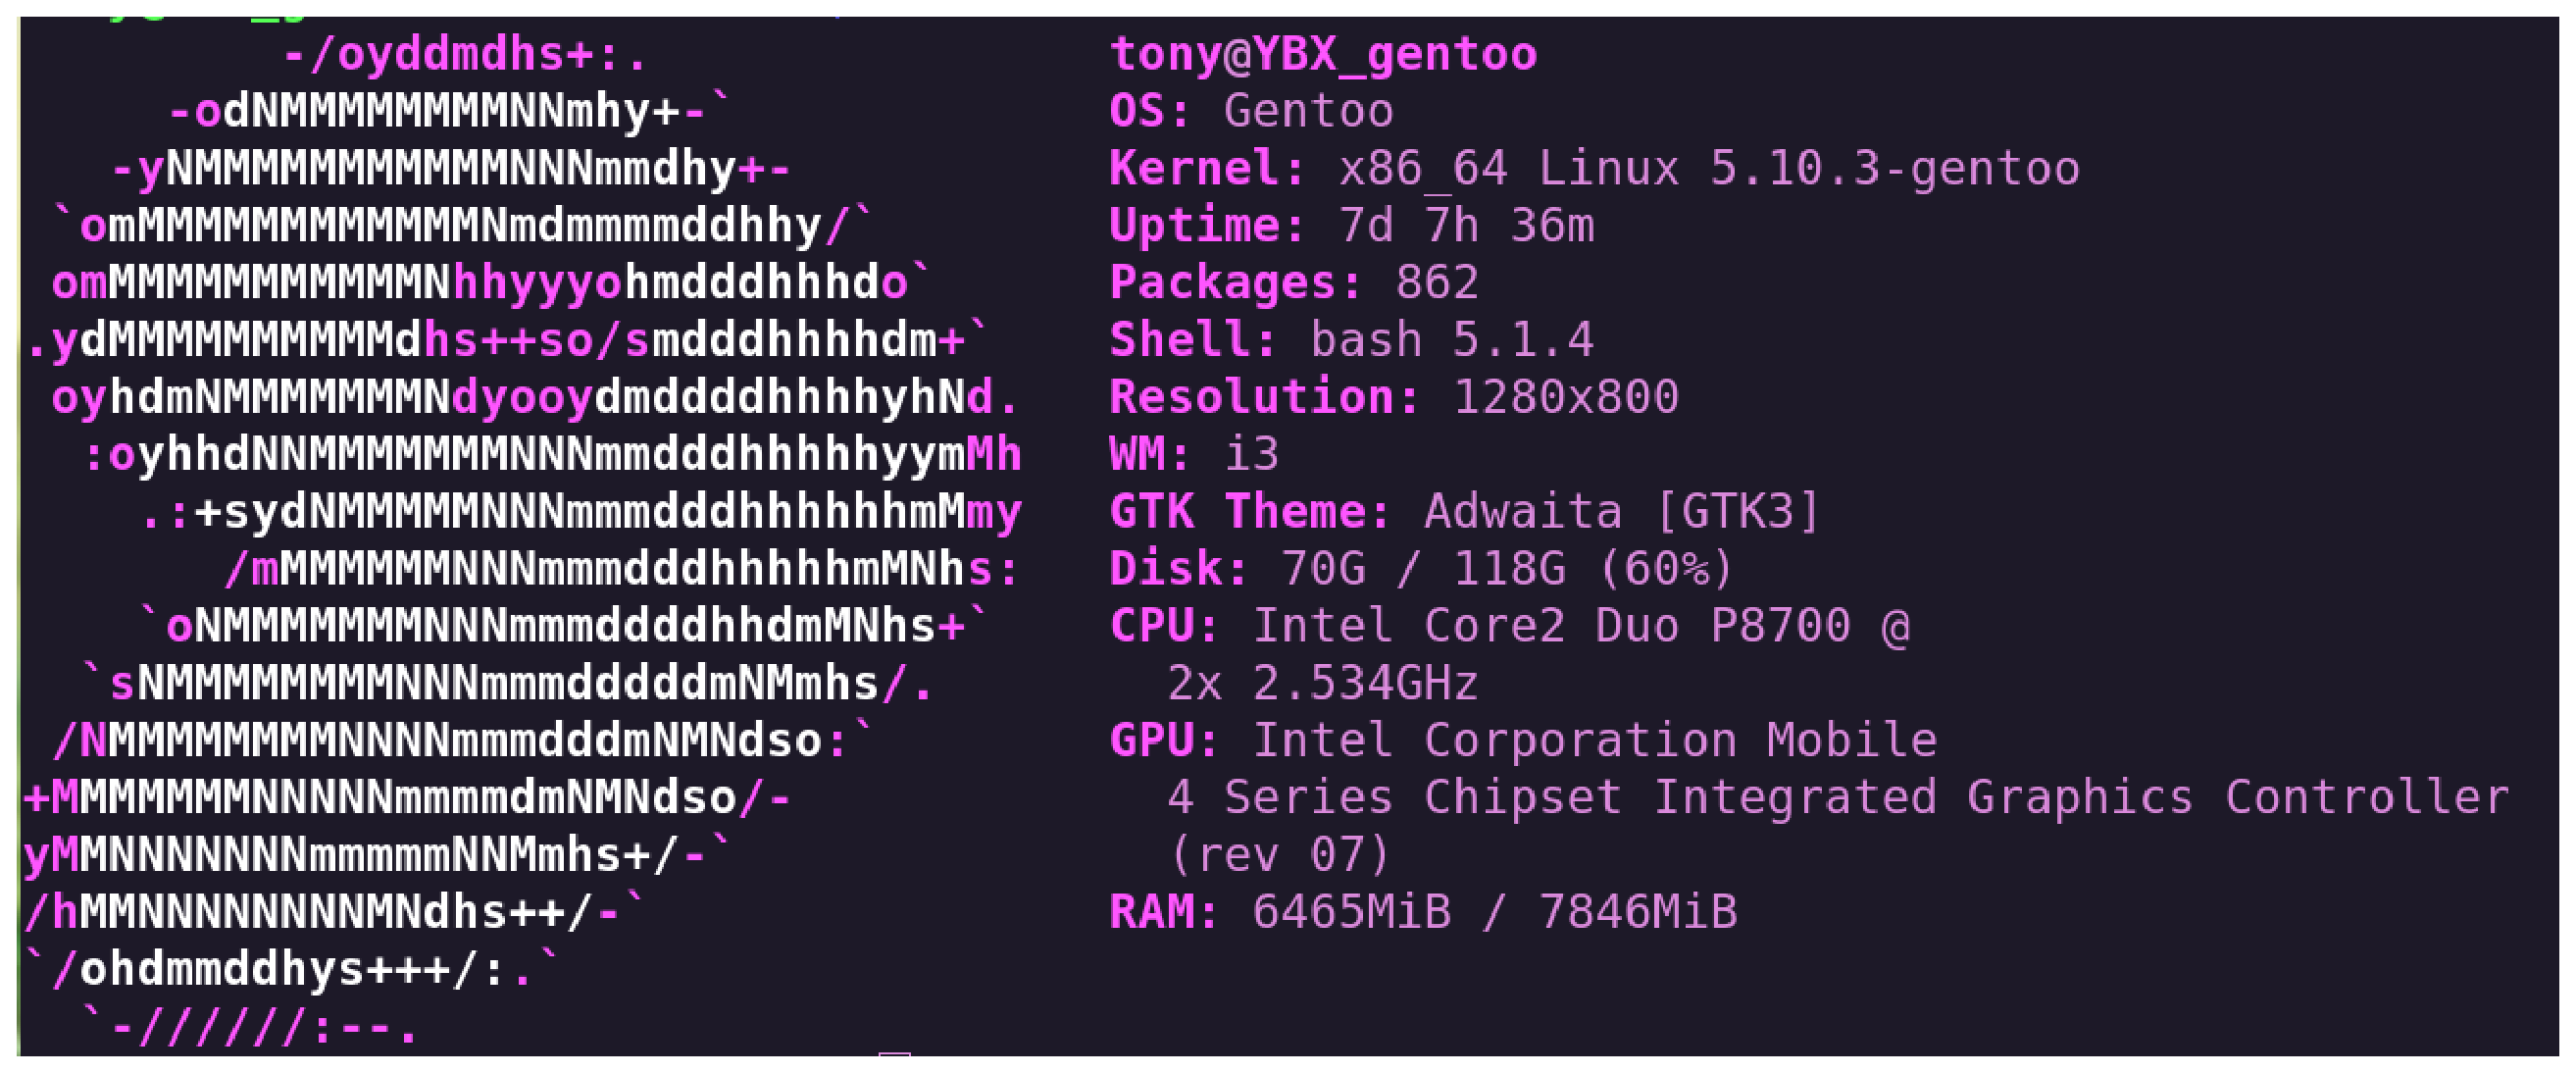
\includegraphics[width=0.8 \textwidth]{figs/Process/gentoo_Logo.eps}
  \caption{实验操作系统}
  \label{fig:gentoo} %设置图形引用名称
\end{figure}

\subsubsection{交叉工具链的准备}
本文我使用的是GNU提供的交叉工具链,实验前需要安装并配置好实验所需的工具链,并根据仓库的 README.md 文档,在x86平台交叉编译出 RISC-V 所需的工具链, 并进行安装与配置  \cite{riscv-binutils-gdb} \cite{riscv-dejagnu} \cite{riscv-gcc} \cite{riscv-glibc} \cite{riscv-newlib} \cite{riscv-pk} ,本实验所需的各种GNU工具链软件信息如图\ref{fig:info}。

其中,这些仓库比较多一个一个下载比较浪费时间,而且加起来也很大,所以后来发现在执行的时候可以递归下载 riscv-gnu-toolchain \cite{riscv-gnu-toolchain} ,可以一次将全部所需的工具链下载完成,最后在使用 Autotool 进行 configure,并根据自身机器进行配置,详细内容可见附录B。


\begin{figure}[htbp]
  \centering %居中显示
  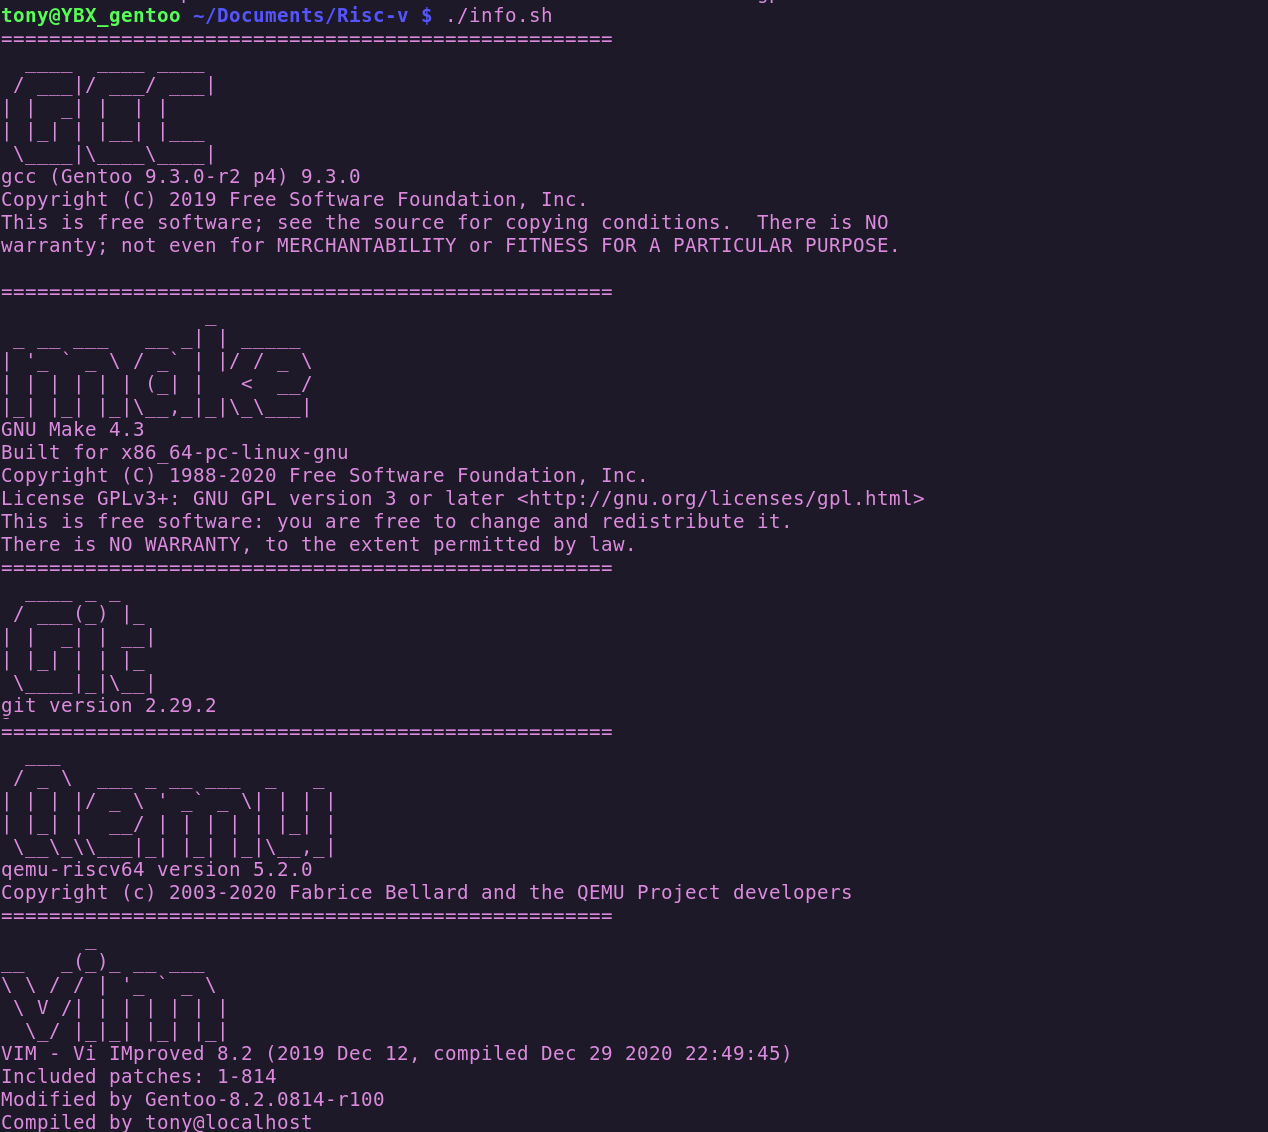
\includegraphics[width=1.0 \textwidth]{figs/Process/info.png}
  \caption{实验所需软件信息}
  \label{fig:info} %设置图形引用名称
\end{figure}

\subsection{Qemu \& KVM搭建}
因为使用的系统环境是 Gentoo Linux ,所以根据 Gentoo 官方的 Wiki 手册中 Qemu 部分来按照步骤完成即可 \cite{GentooQemu} , 主要修改系统中的 USE 来支持RISC-V \cite{KVM安装与配置} ,详细内容可见已经录制好的视频《第一次安装配置Gentoo》\cite{第一次安装配置Gentoo}中 Qemu \& KVM 部分。
% 
\subsection{移植过程介绍}
Linux在 v5.0 以后,既然内核已经可以支持RISC-V,这样只需要在使用 make menuconfig 配置内核的时候加上支持RISC-V的参数,并在make的时候加上选项 ARCH=riscv ,并指定需要的交叉编译器参数即可, 当然编译不是一次就能成功的, 可能已经编译很长时间最后还是失败了, 但是可以根据日志来进行修改配置文件, 最后其他设置就具体情况具体分析即可。

\subsection{制作 BootLoader——BBL(Berkeley Boot Loader)}
这里是根据 riscv-pk \cite{riscv-pk} 中 README.md 的步骤完成实现的。

需要注意的是在编译的时候需要指定risc-v linux Kernel 的最原始未压缩的内核文件—— vmlinux , 完成编译 BootLoader, 具体实现脚本可见附录B。

\subsection{创建根文件系统}
busybon使用了 riscv-qemu 的 virtio-net 与 virtio-block。首先需要使用 qemu-img 生成一块磁盘,用于分区,并存放文件系统。

在busybear的说明文档中有提到可以使用 busybox  来制作文件系统,参考busybox的手册 \cite{busybox} 可以完成其安装配置,并让其完美的运行在Qemu上。

对于文件系统格式化,采用通用的ext4格式,挂载到临时文件夹,并创建根目录所需的一切结构文件夹,结束后要将临时文件夹删除。

\subsection{配置SSH服务}
考虑目前的系统比较简单不完善,所以考虑使用SSH来进行访问与操作。

在给系统实现 SSH 服务时,这里使用dropbear 来实现提供对简单的risc-v 操作系统的SSH服务,其实我想实现SSH操作并且可以外部访问,根据 Dropbear的官方文档\cite{Dropbear} 实现安装与运行操作。

\subsection{最终效果}
最终启动结果如图\ref{fig:success}所示,可以支持SSH访问,如图\ref{fig:ssh_transparent}所示,并且可以执行程序如图\ref{fig:run_truth}所示。
\begin{figure}[htbp]
  \centering %居中显示
  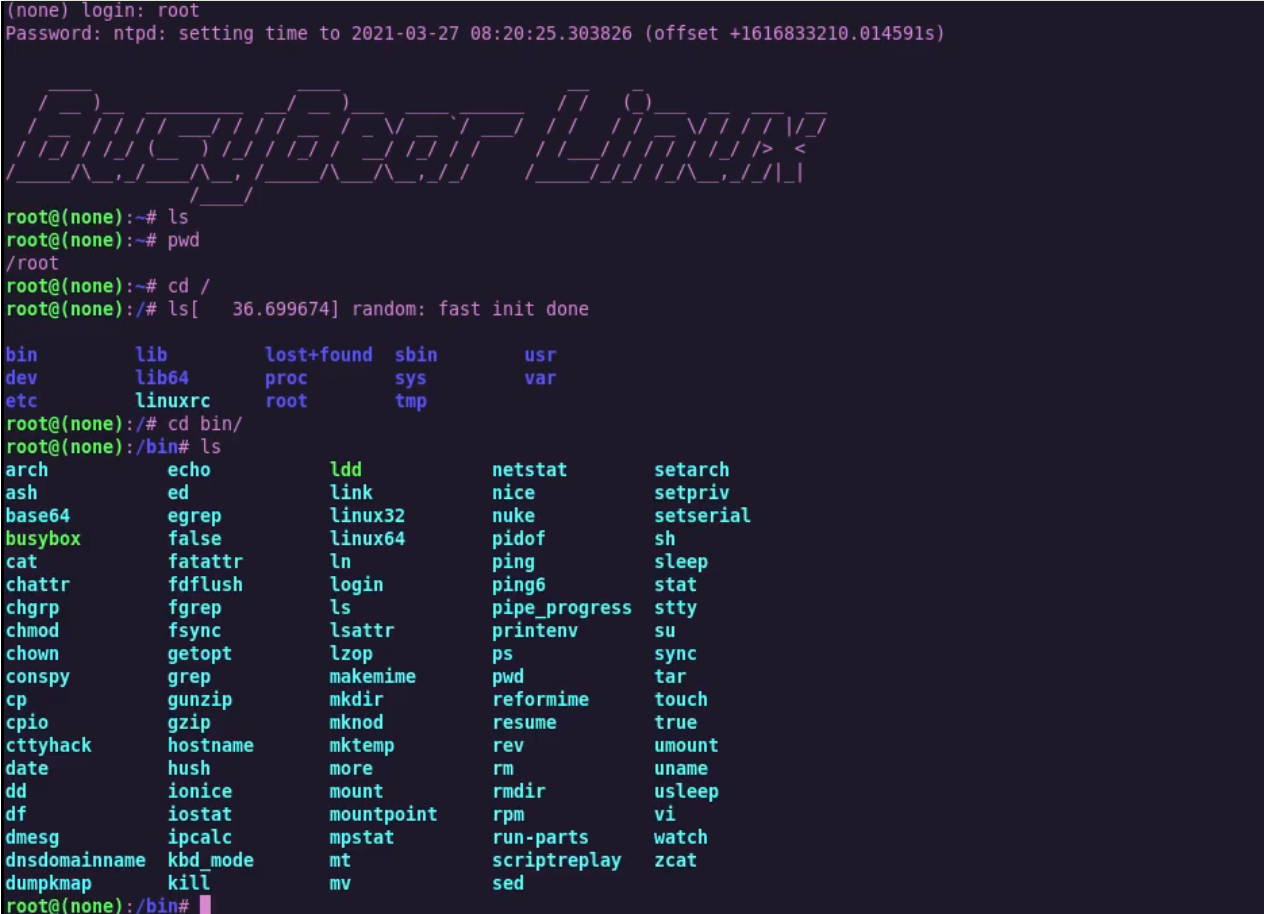
\includegraphics[width=0.9 \textwidth]{figs/Process/success.png}
  \caption{运行成功}
  \label{fig:success} %设置图形引用名称
\end{figure}

\begin{figure}[htbp]
  \centering %居中显示
  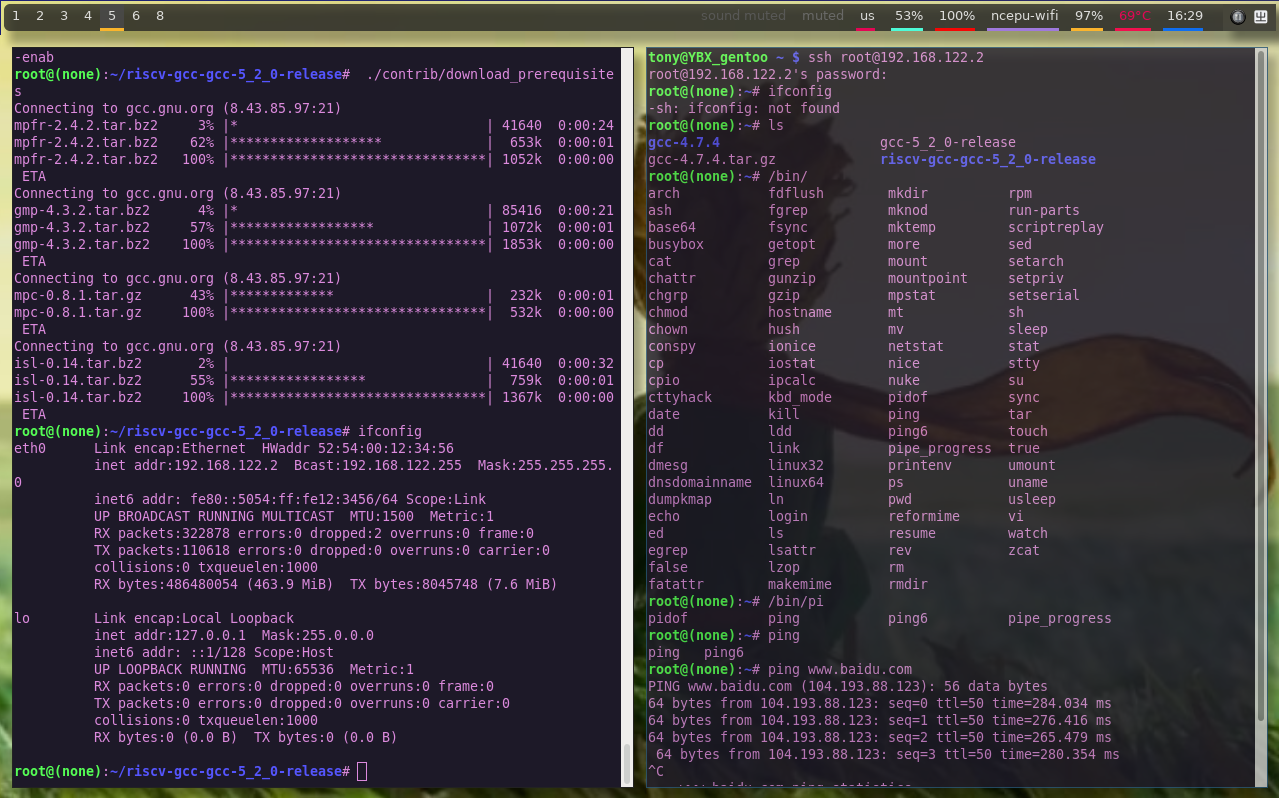
\includegraphics[width=1.0 \textwidth]{figs/Process/ssh_transparent.png}
  \caption{支持SSH网络连接}
  \label{fig:ssh_transparent} %设置图形引用名称
\end{figure}

为了表明自己实验成功是 RISC-V 的, 实现编译好一个 RISC-V 的程序, 来验证该操作系统能否正常的使用, ./truth.riscv 是实现编译好的一个演示程序, 运行结果如图\ref{fig:run_truth}所示,可以正常运行成功。

\begin{figure}[htbp]
  \centering %居中显示
  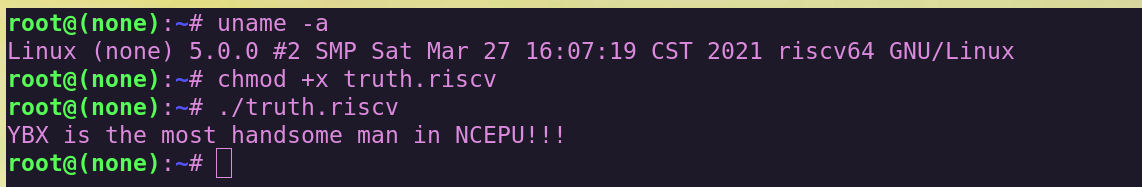
\includegraphics[width=0.9 \textwidth]{figs/Process/run_truth.png}
  \caption{运行程序}
  \label{fig:run_truth} %设置图形引用名称
\end{figure}








\newpage % 相关工作
% 本章节介绍与前人的比较
\section{与前人比较}
虽然本实验以前有人在Github上已经实现了,并且发布成项目 \cite{BusyBear} ,但是该实验工程已经四年多没有更新,在根据 README.md 文档重新复现该实验的时候,发现其中很多步骤已经失效了,而且运行很多步骤也会报错,但这些问题并不算什么的,我依旧可以凭借着这几年下来所学的知识进行解决,并成功运行一个演示程序。

比前人改进的地方就是全部软件更新到现在主流版本,修改了一些步骤上遇到的错误,以及解决遇到的一系列问题。

\subsection{收获}
通过该课程设计,让我对Qemu有了更深的理解,再加上对操作系统底层有更深的理解,更深体会到编译工具的熟练使用。

\subsection{不足}
虽然,本文已经可以运行一个程序,但是目前还有如下问题:(1)图形界面,就是用户需要使用图形界面的,这样可以更加方便用户使用,但是目前还没有想清楚如何添加图形界面方法;(2)需要做横向对比,和MIPS,ARM比较,看一下RISC-V的平台会提高多少性能;(3)其实这个也不算标准的移植,成功运行了,但是不代表日后会不会出现函数库,以及依赖的问题;

\newpage  %与前人比较
% 总结
\section{总结}
本文仅仅是利用本科所学知识来进行的一次应用,就是将Linux移植到risc-v平台上,涉及到内容比较基础,主要目的是通过本毕设将大学的计算机组成原理,操作系统,计算机体系结构来进行全方面的强化,并将理论与实践相结合,最后希望我的一点探索努力可以更好的完善我国在计算机底层领域的长足发展。

\newpage %总结
%--------------------------------------------------------------------------------
%% 参考文献
\begin{sloppypar} %文字超出边界的处理方法 
\normalsize
\songti
\bibliographystyle{gbt7714-2005}
\bibliography{Ref}
\addcontentsline{toc}{section}{\heiti{\Large{参考文献}}}
\end{sloppypar}
%\bibliographystyle{plain}指定参考文献的呈现方式,常见的预设样式的可选项有8种,分别是:
%% 1. plain,按字母的顺序排列,比较次序为作者、年度和标题;
%% 2. unsrt,样式同plain,只是按照引用的先后排序;
%% 3. alpha,用作者名首字母+年份后两位作标号,以字母顺序排序;
%% 4. abbrv,类似plain,将月份全拼改为缩写,更显紧凑;
%% 5. ieeetr,国际电气电子工程师协会期刊样式;
%% 6. acm,美国计算机学会期刊样式;
%% 7. siam,美国工业和应用数学学会期刊样式;
%% 8. apalike,美国心理学学会期刊样式;
%%%%%%%%%%%%%%%%%%%%%%%%%%%%%%%%%%%%%%%%%%%%%%%%%%%%%%%%%%%%%
%--------------------------------------------------------------------------------
%% 附录
% 附录

%\CTEXsetup[name={附录,},format={\raggedright\songti\zihao{4}},aftername={\enspace},beforeskip={12bp},afterskip={6bp}]{subsubsection}

\renewcommand\thesection{附录\Alph{subsubsection}}

\newpage
\renewcommand{\abstractname}{\heiti{\zihao{-2} {附\quad \quad \quad \quad 录}}}
\begin{abstract}
\phantomsection
\addcontentsline{toc}{section}{\heiti{\Large{附 \quad \quad 录}}}    

%%%%%%%%%%%%%%%%%%%%%%%%%%%%%%%%%%%%%%%%%
%% 附录A
~\\
\begin{center}
    \heiti{\zihao{-2} {附录A}}
\end{center}
\phantomsection
\addcontentsline{toc}{subsection}{\songti{\large{附录A}}}    
\setlength{\baselineskip}{20pt} %行距20磅
\begin{sloppypar} %文字超出边界的处理方法 
{\zihao{-4} {
    关于Gentoo Linux的部分配置请见:https://www.bilibili.com/video/BV1ny4y1i7G6 的视频演示。

    关于本毕设的实验请见:https://www.bilibili.com/video/BV1QU4y1H7AE。
    
}}

%%%%%%%%%%%%%%%%%%%%%%%%%%%%%%%%%%%%%%%%%
%% 附录B
~\\
\begin{center}
    \heiti{\zihao{-2} {附录B}}
\end{center}
\phantomsection
\addcontentsline{toc}{subsection}{\songti{\large{附录B}}}   
\subsection*{修改USE Flags并安装}
\begin{lstlisting}
# vim /etc/portage/make.conf
QEMU_SOFTMMU_TARGETS="riscv32 risc64"
QEMU_USER_TARGETS="x86_64"

# vim /etc/portage/package.use
app-emulation/qemu qemu_softmmu_targets_arm qemu_softmmu_targets_x86_64
                 qemu_softmmu_targets_sparc
app-emulation/qemu qemu_user_targets_x86_64

% 进行安装
# emerge --ask app-emulation/qemu -y
\end{lstlisting}


\subsection*{安装GNU工具链}
\begin{lstlisting}
mkdir YBX-bishe
cd YBX-bishe/
# 拉取 gnu-toolchain
git clone --recursive https://github.com/riscv/riscv-gnu-toolchain

# 编译生成 RISC-V newlib & Linux toolchains
cd riscv-gnu-toolchain
./configure --prefix=/opt/riscv --enable-multilib
make newlib -j5
make linux -j5
export PATH=$PATH:/opt/riscv/bin
export RISCV=/opt/risc
$
\end{lstlisting}

\subsection*{创建根文件系统}
\begin{lstlisting}
cd ..
git clone https://github.com/michaeljclark/busybear-linux.git
cd busybear-linux
make -j5
\end{lstlisting}

但是这没完,因为busybear会自动帮你下载好 busybox 但是需要自己进行解压和编译

\begin{lstlisting}
CROSS_COMPILE=riscv{{bits}}-unknown-linux-gnu- make menuconfig
CROSS_COMPILE=riscv{{bits}}-unknown-linux-gnu- make
\end{lstlisting}

下面咱们就要制做最小文件系统
\begin{lstlisting}
qemu-img create rootfs.img  1g
mkfs.ext4 rootfs.img
mkdir rootfs
sudo mount -o loop rootfs.img  rootfs
cd rootfs
sudo cp -r ../busyboxsource/_install/* .
sudo mkdir proc sys dev etc etc/init.d
cd etc/init.d/
sudo touch rcS
sudo vi rcS
#!/bin/sh
mount -t proc none /proc
mount -t sysfs none /sys
/sbin/mdev -s

sudo mod +x rcS
sudo umount rootfs
\end{lstlisting}

\subsection*{构建Linux内核}
\begin{lstlisting}
git clone https://github.com/torvalds/linux
cd linux
git checkout v5.4
make ARCH=riscv CROSS_COMPILE=riscv64-unknown-linux-gnu- defconfig
make ARCH=riscv CROSS_COMPILE=riscv64-unknown-linux-gnu-
\end{lstlisting}

\subsection*{制作BootLoader——BBL(Berkeley Boot Loader)}
\begin{lstlisting}
cd..
git clone https://github.com/riscv/riscv-pk.git
cd riscv-pk
mkdir build
cd build
../configure \
> --enable-logo \
> --host=riscv64-unknown-elf \
> --with-payload=../../riscv-linux/vmlinux

make -j8
\end{lstlisting}

\subsection*{编写各种所需脚本}
\begin{lstlisting}
cd ..
mkdir Running
cd Running
\end{lstlisting}
创建KVM启动脚本
\begin{lstlisting}
vim open_kvm
#!/bin/sh
sudo /etc/init.d/libvirtd start
sudo virsh net-start default  #开启网络服务
\end{lstlisting}

创建KVM关闭脚本
\begin{lstlisting}
sudo virsh net-destory default
sudo /etc/init.d/libvirtd stop
\end{lstlisting}


创建网络启动脚本
\begin{lstlisting}
#!/bin/sh
brctl addif virbr0 $1
ifconfig $1 up
\end{lstlisting}

创建网络关闭脚本
\begin{lstlisting}
#!/bin/sh
ifconfig $1 down
brctl delif virbr0 $1
\end{lstlisting}

创建程序运行脚本
\begin{lstlisting}
#!/bin/sh
# QEMU 5.2以后.模拟器内部集成了OpenSBI
sudo qemu-system-riscv64 \
  -nographic -machine virt \
  -m 1024M \
  -kernel bbl \
  -kernel ~/Documents/Risc-v/busybear-linux/build/linux-5.0/arch
                  /riscv/boot/Image \
  -drive file=busybear.bin,format=raw,id=hd0 \
  -device virtio-blk-device,drive=hd0 \
  -device virtio-net-device,netdev=net0 \
  -netdev type=tap,script=./ifup.sh,downscript=./ifdown.sh,id=net0 \
  -append "root=/dev/vda ro console=ttyS0"
\end{lstlisting}

\subsection*{运行}
\begin{lstlisting}
./Running.sh
\end{lstlisting}


\end{sloppypar}
\end{abstract}
\newpage
%--------------------------------------------------------------------------------
% %% 致谢
% 致谢
\newpage
\renewcommand{\abstractname}{\heiti{\huge{致\quad \quad \quad \quad 谢}}}
\begin{abstract}
\phantomsection
\addcontentsline{toc}{section}{\heiti{\Large{致 \quad \quad 谢}}}    
\setlength{\baselineskip}{20pt} %行距20磅
    {\zihao{-4}{ 首先,我非常感谢我的家长,从小到大对我的殷勤付出,最终我才能有今天的收获,是他们的坚持不懈才让本因高考没有考上重点大学的我尽可能没有堕落下去;其次要感谢大学这群功利现实冷酷有没有人情的学生们,他们就是我的好教员,他们用他们冷漠自私让我明白一个道理“落后就要挨打,贫穷就要挨饿,失语就要挨骂”,只有站起来而不是跪下去才会有美好的未来;然后,要感谢毛泽东,邓小平等那些思想领袖,从他们哪里我学到了很多,大学之前没接触过计算机让我刚来的时候挂了不少课也被与预警过,但是面对这样的内外交迫的处境,“速战论”激进思想与“亡国论”的消极思想是不可取的,应该要打持久战,这是一场没有硝烟的战争,大致可划分三个阶段——“战略防御、战略相持、战略反攻”,要团结一切力量,积小胜为大胜,面对帝国主义和资产阶级那种腐朽、堕落和淫乱不堪的作风态度要坚定,最后我在大二结束的暑假就自学完本科全部的内容,并大三顺利地进入战略反攻阶段时,摧枯拉朽般把大一大二欠下的全部课程以及大三大四的课程一并补齐。最后还是要走一条具有自身特色的发展路线,要将理论与实践相结合,鞋子合不合脚自己穿了才知道;最后我要感谢琚赟老师,首先他并不像其他老师那样因为我大一大二基础差而区别对待,其次也没有“好心”地劝过“你学习不好的原因就是因为不努力学习,要抓紧学习”仅仅喊口号并没有提出解决方案,更没有说类似“我当了这么多年老师,你不是我见过聪明的学生”的话,而是采用基层民主制度,让我充分发挥自主的能动性,而不像奴才一样必须被用鞭子催着赶着让去做一件事。

高考刚结束,那时的我们还有梦,还有热情,还有诗和远方;畅想着关于自己,关于未来,关于一场穿越时空的旅行。 而如今我们深夜饮酒, 杯子碰到一起, 都是梦破碎的声音。

    ~\\
\indent   在这四年里 \\
\indent   我知道这个世界很美好,可是我却感受不到!\\
\indent   我知道阳光很暖,风很舒服,可是我更希望你们能被这样的温柔感化!\\    
\indent   这个世间一切都那么美好,希望人与人之间也能像风和太阳那般!\\
\indent   我也知道爱情很美好,可是它不会降临在我身上,所以我希望你们能拥有!\\
\indent   ……\\
\indent   一切的一切我都知道,但是它们都不属于我!\\

\indent   从明天开始,要做一个幸福的人\\ 
\indent   我要闻一闻花的芬芳\\
\indent   我要望一望璀璨的夜空\\
\indent   我要享受一下微风拂面的惬意\\ 
\indent   我要给每一条河每一座山都取一个温暖的名字\\ 
\indent   从明天开始,要告诉每一个关心我的人我的幸福\\ 
\indent   我要祝福每一个陌生人在尘世中过得开心,有光明的前程\\ 
\indent   我愿面朝大海,春暖花开\\ 

}}
\end{abstract}
\newpage
\end{document}
